\batchmode
\documentclass[twoside]{book}

% Packages required by doxygen
\usepackage{fixltx2e}
\usepackage{calc}
\usepackage{doxygen}
\usepackage[export]{adjustbox} % also loads graphicx
\usepackage{graphicx}
\usepackage[utf8]{inputenc}
\usepackage{makeidx}
\usepackage{multicol}
\usepackage{multirow}
\PassOptionsToPackage{warn}{textcomp}
\usepackage{textcomp}
\usepackage[nointegrals]{wasysym}
\usepackage[table]{xcolor}

% Font selection
\usepackage[T1]{fontenc}
\usepackage[scaled=.90]{helvet}
\usepackage{courier}
\usepackage{amssymb}
\usepackage{sectsty}
\renewcommand{\familydefault}{\sfdefault}
\allsectionsfont{%
  \fontseries{bc}\selectfont%
  \color{darkgray}%
}
\renewcommand{\DoxyLabelFont}{%
  \fontseries{bc}\selectfont%
  \color{darkgray}%
}
\newcommand{\+}{\discretionary{\mbox{\scriptsize$\hookleftarrow$}}{}{}}

% Page & text layout
\usepackage{geometry}
\geometry{%
  a4paper,%
  top=2.5cm,%
  bottom=2.5cm,%
  left=2.5cm,%
  right=2.5cm%
}
\tolerance=750
\hfuzz=15pt
\hbadness=750
\setlength{\emergencystretch}{15pt}
\setlength{\parindent}{0cm}
\setlength{\parskip}{3ex plus 2ex minus 2ex}
\makeatletter
\renewcommand{\paragraph}{%
  \@startsection{paragraph}{4}{0ex}{-1.0ex}{1.0ex}{%
    \normalfont\normalsize\bfseries\SS@parafont%
  }%
}
\renewcommand{\subparagraph}{%
  \@startsection{subparagraph}{5}{0ex}{-1.0ex}{1.0ex}{%
    \normalfont\normalsize\bfseries\SS@subparafont%
  }%
}
\makeatother

% Headers & footers
\usepackage{fancyhdr}
\pagestyle{fancyplain}
\fancyhead[LE]{\fancyplain{}{\bfseries\thepage}}
\fancyhead[CE]{\fancyplain{}{}}
\fancyhead[RE]{\fancyplain{}{\bfseries\leftmark}}
\fancyhead[LO]{\fancyplain{}{\bfseries\rightmark}}
\fancyhead[CO]{\fancyplain{}{}}
\fancyhead[RO]{\fancyplain{}{\bfseries\thepage}}
\fancyfoot[LE]{\fancyplain{}{}}
\fancyfoot[CE]{\fancyplain{}{}}
\fancyfoot[RE]{\fancyplain{}{\bfseries\scriptsize Generated by Doxygen }}
\fancyfoot[LO]{\fancyplain{}{\bfseries\scriptsize Generated by Doxygen }}
\fancyfoot[CO]{\fancyplain{}{}}
\fancyfoot[RO]{\fancyplain{}{}}
\renewcommand{\footrulewidth}{0.4pt}
\renewcommand{\chaptermark}[1]{%
  \markboth{#1}{}%
}
\renewcommand{\sectionmark}[1]{%
  \markright{\thesection\ #1}%
}

% Indices & bibliography
\usepackage{natbib}
\usepackage[titles]{tocloft}
\setcounter{tocdepth}{3}
\setcounter{secnumdepth}{5}
\makeindex

% Hyperlinks (required, but should be loaded last)
\usepackage{ifpdf}
\ifpdf
  \usepackage[pdftex,pagebackref=true]{hyperref}
\else
  \usepackage[ps2pdf,pagebackref=true]{hyperref}
\fi
\hypersetup{%
  colorlinks=true,%
  linkcolor=blue,%
  citecolor=blue,%
  unicode%
}

% Custom commands
\newcommand{\clearemptydoublepage}{%
  \newpage{\pagestyle{empty}\cleardoublepage}%
}

\usepackage{caption}
\captionsetup{labelsep=space,justification=centering,font={bf},singlelinecheck=off,skip=4pt,position=top}

%===== C O N T E N T S =====

\begin{document}

% Titlepage & ToC
\hypersetup{pageanchor=false,
             bookmarksnumbered=true
            }
\pagenumbering{alph}
\pagenumbering{arabic}
\hypersetup{pageanchor=true}

%--- Begin generated contents ---
\chapter{Example problem\+: The Young Laplace equation with contact angle boundary conditions}
\label{index}\hypertarget{index}{}\hypertarget{index_q}{}\section{A few quick questions...}\label{index_q}
Since {\ttfamily oomph-\/lib} is developed as open-\/source software, any evidence that the code is being downloaded and used is very helpful for us as it helps to justify our continued work on this project.

We would therefore be extremely grateful if you could provide the information requested in the form below. Pressing the \char`\"{}submit\char`\"{} button will get you to the actual download page.

{\bfseries Note\+:} 
\begin{DoxyItemize}
\item All information will be treated as confidential. 
\item If you provide your email address and check the appropriate box we will add you to our mailing list to inform you of upgrades and bug fixes to the code. Rest assured that the mailing list is {\bfseries very low volume} -- we have better things to do than to bombard you with email. 
\item If you still feel reluctant to provide any of the information requested, feel free to enter some dummy input. The form will check that {\bfseries some} information has been entered but entering your name as \char`\"{}\+Joe Cool\char`\"{} is perfectly acceptable -- this is to discourage people from not providing the information simply because they are too lazy to type... 
\end{DoxyItemize}



 







 

 \hypertarget{index_pdf}{}\section{P\+D\+F file}\label{index_pdf}
A \href{../latex/refman.pdf}{\tt pdf version} of this document is available. \end{document}

\chapter{Namespace Index}
\section{Namespace List}
Here is a list of all namespaces with brief descriptions\+:\begin{DoxyCompactList}
\item\contentsline{section}{\hyperlink{namespaceGlobal__Physical__Variables}{Global\+\_\+\+Physical\+\_\+\+Variables} \\*Global variables that represent physical properties }{\pageref{namespaceGlobal__Physical__Variables}}{}
\item\contentsline{section}{\hyperlink{namespaceoomph}{oomph} }{\pageref{namespaceoomph}}{}
\item\contentsline{section}{\hyperlink{namespacePhysical__Variables}{Physical\+\_\+\+Variables} \\*Namespace for the solution of 2D linear shell equation }{\pageref{namespacePhysical__Variables}}{}
\end{DoxyCompactList}

\chapter{Hierarchical Index}
\section{Class Hierarchy}
This inheritance list is sorted roughly, but not completely, alphabetically\+:\begin{DoxyCompactList}
\item Problem\begin{DoxyCompactList}
\item \contentsline{section}{Unstructured\+Solid\+Problem$<$ E\+L\+E\+M\+E\+NT $>$}{\pageref{classUnstructuredSolidProblem}}{}
\end{DoxyCompactList}
\end{DoxyCompactList}

\chapter{Class Index}
\section{Class List}
Here are the classes, structs, unions and interfaces with brief descriptions\+:\begin{DoxyCompactList}
\item\contentsline{section}{\hyperlink{classPMLProblem}{P\+M\+L\+Problem$<$ E\+L\+E\+M\+E\+N\+T $>$} }{\pageref{classPMLProblem}}{}
\item\contentsline{section}{\hyperlink{classGlobalParameters_1_1TestPMLMapping}{Global\+Parameters\+::\+Test\+P\+M\+L\+Mapping} }{\pageref{classGlobalParameters_1_1TestPMLMapping}}{}
\end{DoxyCompactList}

\chapter{File Index}
\section{File List}
Here is a list of all files with brief descriptions\+:\begin{DoxyCompactList}
\item\contentsline{section}{\hyperlink{jeffery__orbit_8cc}{jeffery\+\_\+orbit.\+cc} }{\pageref{jeffery__orbit_8cc}}{}
\item\contentsline{section}{\hyperlink{jeffery__orbit_8txt__doxygenified_8h}{jeffery\+\_\+orbit.\+txt\+\_\+doxygenified.\+h} }{\pageref{jeffery__orbit_8txt__doxygenified_8h}}{}
\item\contentsline{section}{\hyperlink{my__taylor__hood__elements_8h}{my\+\_\+taylor\+\_\+hood\+\_\+elements.\+h} }{\pageref{my__taylor__hood__elements_8h}}{}
\end{DoxyCompactList}

\chapter{Namespace Documentation}
\hypertarget{namespaceGlobalParameters}{}\section{Global\+Parameters Namespace Reference}
\label{namespaceGlobalParameters}\index{Global\+Parameters@{Global\+Parameters}}


Namespace for \char`\"{}global\char`\"{} problem parameters.  


\subsection*{Enumerations}
\begin{DoxyCompactItemize}
\item 
enum \hyperlink{namespaceGlobalParameters_adde04e4243b82e3d4bd2f82d37a2d6bf}{Cases} \{ \hyperlink{namespaceGlobalParameters_adde04e4243b82e3d4bd2f82d37a2d6bfac08080f634c714da38f1122301eafda7}{Spherical\+\_\+cap\+\_\+in\+\_\+cylinder\+\_\+pinned}, 
\hyperlink{namespaceGlobalParameters_adde04e4243b82e3d4bd2f82d37a2d6bfa28147edc9cfc06038f2a7deaf8890558}{All\+\_\+pinned}, 
\hyperlink{namespaceGlobalParameters_adde04e4243b82e3d4bd2f82d37a2d6bfa1e6d2261f2fa0541d57b5a0a8c044ddc}{Barrel\+\_\+shape}, 
\hyperlink{namespaceGlobalParameters_adde04e4243b82e3d4bd2f82d37a2d6bfa89cfbba408c0774e0b9024baa187dfb8}{T\+\_\+junction\+\_\+with\+\_\+nonzero\+\_\+contact\+\_\+angle}
 \}\begin{DoxyCompactList}\small\item\em Enumeration for the possible cases. \end{DoxyCompactList}
\end{DoxyCompactItemize}
\subsection*{Functions}
\begin{DoxyCompactItemize}
\item 
double \hyperlink{namespaceGlobalParameters_a4571d41514b16946dd31d075d44c5593}{get\+\_\+exact\+\_\+kappa} ()
\begin{DoxyCompactList}\small\item\em Exact kappa. \end{DoxyCompactList}\item 
void \hyperlink{namespaceGlobalParameters_ac81daf87f8d3f075d9fd108427e70c4f}{spine\+\_\+base\+\_\+function} (const Vector$<$ double $>$ \&x, Vector$<$ double $>$ \&spine\+\_\+B, Vector$<$ Vector$<$ double $>$ $>$ \&dspine\+\_\+B)
\begin{DoxyCompactList}\small\item\em Spine basis\+: The position vector to the basis of the spine as a function of the two coordinates x\+\_\+1 and x\+\_\+2, and its derivatives w.\+r.\+t. to these coordinates. dspine\+\_\+B\mbox{[}i\mbox{]}\mbox{[}j\mbox{]} = d spine\+\_\+B\mbox{[}j\mbox{]} / dx\+\_\+i Spines start in the (x\+\_\+1,x\+\_\+2) plane at (x\+\_\+1,x\+\_\+2). \end{DoxyCompactList}\item 
void \hyperlink{namespaceGlobalParameters_a82df8c67f58e78a236fb6a0cc8bf8284}{spine\+\_\+function} (const Vector$<$ double $>$ \&x, Vector$<$ double $>$ \&spine, Vector$<$ Vector$<$ double $>$ $>$ \&dspine)
\begin{DoxyCompactList}\small\item\em Spine\+: The spine vector field as a function of the two coordinates x\+\_\+1 and x\+\_\+2, and its derivatives w.\+r.\+t. to these coordinates\+: dspine\mbox{[}i\mbox{]}\mbox{[}j\mbox{]} = d spine\mbox{[}j\mbox{]} / dx\+\_\+i. \end{DoxyCompactList}\item 
void \hyperlink{namespaceGlobalParameters_aedbc21f2c81d445634badfc5cdd77436}{setup\+\_\+dependent\+\_\+parameters\+\_\+and\+\_\+sanity\+\_\+check} ()
\begin{DoxyCompactList}\small\item\em Setup dependent parameters and perform sanity check. \end{DoxyCompactList}\end{DoxyCompactItemize}
\subsection*{Variables}
\begin{DoxyCompactItemize}
\item 
double \hyperlink{namespaceGlobalParameters_a3731f24a02ce4f306d65a9a488f85c96}{Controlled\+\_\+height} = 0.\+0
\begin{DoxyCompactList}\small\item\em Height control value. \end{DoxyCompactList}\item 
double \hyperlink{namespaceGlobalParameters_ae8fa7610a34b7a2a8223eade99a5c22f}{Alpha\+\_\+min} = Mathematical\+Constants\+::\+Pi/2.\+0$\ast$1.\+5
\begin{DoxyCompactList}\small\item\em Min. spine angle against horizontal plane. \end{DoxyCompactList}\item 
double \hyperlink{namespaceGlobalParameters_a19d04a02b0b5ef5c72e9c30d822e4dc7}{Alpha\+\_\+max} = Mathematical\+Constants\+::\+Pi/2.\+0$\ast$0.\+5
\begin{DoxyCompactList}\small\item\em Max. spine angle against horizontal plane. \end{DoxyCompactList}\item 
bool \hyperlink{namespaceGlobalParameters_a7cd7766fae9d0ca421d7e24677be3131}{Use\+\_\+spines} = true
\begin{DoxyCompactList}\small\item\em Use spines (true) or not (false) \end{DoxyCompactList}\item 
bool \hyperlink{namespaceGlobalParameters_a624713d35bc418b2d5fa79f4d385a27a}{Use\+\_\+height\+\_\+control} = true
\begin{DoxyCompactList}\small\item\em Use height control (true) or not (false)? \end{DoxyCompactList}\item 
int \hyperlink{namespaceGlobalParameters_aeb4257eec7a4c5a92e2b88e93248a201}{Case} = \hyperlink{namespaceGlobalParameters_adde04e4243b82e3d4bd2f82d37a2d6bfa28147edc9cfc06038f2a7deaf8890558}{All\+\_\+pinned}
\begin{DoxyCompactList}\small\item\em What case are we considering\+: Choose one from the enumeration Cases. \end{DoxyCompactList}\item 
double \hyperlink{namespaceGlobalParameters_adb0a994119055242fcc762cac5edc317}{Gamma} = Mathematical\+Constants\+::\+Pi/4.\+0
\begin{DoxyCompactList}\small\item\em Contact angle and its cos (dependent parameter -- is reassigned) \end{DoxyCompactList}\item 
double \hyperlink{namespaceGlobalParameters_ae982fcb894e82c683d07d3c2fbbead3d}{Cos\+\_\+gamma} =cos(\hyperlink{namespaceGlobalParameters_adb0a994119055242fcc762cac5edc317}{Gamma})
\begin{DoxyCompactList}\small\item\em Cos of contact angle. \end{DoxyCompactList}\item 
Data $\ast$ \hyperlink{namespaceGlobalParameters_ac6234184cce40ab2c6bec92b37e4ae41}{Kappa\+\_\+pt} = 0
\begin{DoxyCompactList}\small\item\em Pointer to Data object that stores the prescribed curvature. \end{DoxyCompactList}\item 
double \hyperlink{namespaceGlobalParameters_ae7651e73d3f8346da9fcfdbb149bc22e}{Kappa\+\_\+initial} = 0.\+0
\begin{DoxyCompactList}\small\item\em Initial value for kappa. \end{DoxyCompactList}\item 
int \hyperlink{namespaceGlobalParameters_aeb81cc1c282502497ef6df576559b650}{Step\+\_\+sign} = 1
\begin{DoxyCompactList}\small\item\em Increase or decrease the value of the control parameters? \end{DoxyCompactList}\item 
unsigned \hyperlink{namespaceGlobalParameters_aa6c94936d7c81286bb747e14a90d7ba0}{Nsteps} = 5
\begin{DoxyCompactList}\small\item\em Number of steps. \end{DoxyCompactList}\item 
double \hyperlink{namespaceGlobalParameters_a74cc88d6dc206cd556fb12e7e3101032}{Kappa\+\_\+increment} = -\/0.\+05
\begin{DoxyCompactList}\small\item\em Increment for prescribed curvature. \end{DoxyCompactList}\item 
double \hyperlink{namespaceGlobalParameters_a65fe7fd6c6c54d7ba89fab47cd4a9141}{Controlled\+\_\+height\+\_\+increment} = 0.\+1
\begin{DoxyCompactList}\small\item\em Increment for height control. \end{DoxyCompactList}\item 
unsigned \hyperlink{namespaceGlobalParameters_a3a90a762edbce6d2a95456df26e85cea}{Control\+\_\+element} = 0
\item 
double \hyperlink{namespaceGlobalParameters_a36ebf514fdd1e78fff69907b39e25af6}{L\+\_\+x} = 1.\+0
\begin{DoxyCompactList}\small\item\em Length and width of the domain. \end{DoxyCompactList}\item 
double \hyperlink{namespaceGlobalParameters_ac8774b3418c4551091d64ec72c169b2e}{L\+\_\+y} = 1.\+0
\begin{DoxyCompactList}\small\item\em Width of domain. \end{DoxyCompactList}\item 
unsigned \hyperlink{namespaceGlobalParameters_ab020cb50fa321b26e8d2127d2cff23b9}{N\+\_\+x} = 8
\begin{DoxyCompactList}\small\item\em Number of elements in the mesh. \end{DoxyCompactList}\item 
unsigned \hyperlink{namespaceGlobalParameters_a711d6f05552ddaac30bd245ae8bdf878}{N\+\_\+y} = 8
\item 
double \hyperlink{namespaceGlobalParameters_aeb7f1ae574be563e0b603662c6fff5aa}{Beta\+\_\+min} = Mathematical\+Constants\+::\+Pi/2.\+0
\begin{DoxyCompactList}\small\item\em Min. second spine angle against horizontal plane. \end{DoxyCompactList}\item 
double \hyperlink{namespaceGlobalParameters_aa34aff6eb29a2a1245e9ffc2fac42caa}{Beta\+\_\+max} = Mathematical\+Constants\+::\+Pi/2.\+0
\begin{DoxyCompactList}\small\item\em Max. second pine angle against horizontal plane. \end{DoxyCompactList}\item 
bool \hyperlink{namespaceGlobalParameters_a69a238365a4fef33b1abdae287185f3e}{Rotate\+\_\+spines\+\_\+in\+\_\+both\+\_\+directions} = true
\begin{DoxyCompactList}\small\item\em Should the spines rotate in the x and y directions (true)? \end{DoxyCompactList}\end{DoxyCompactItemize}


\subsection{Detailed Description}
Namespace for \char`\"{}global\char`\"{} problem parameters. 

\subsection{Enumeration Type Documentation}
\mbox{\Hypertarget{namespaceGlobalParameters_adde04e4243b82e3d4bd2f82d37a2d6bf}\label{namespaceGlobalParameters_adde04e4243b82e3d4bd2f82d37a2d6bf}} 
\index{Global\+Parameters@{Global\+Parameters}!Cases@{Cases}}
\index{Cases@{Cases}!Global\+Parameters@{Global\+Parameters}}
\subsubsection{\texorpdfstring{Cases}{Cases}}
{\footnotesize\ttfamily enum \hyperlink{namespaceGlobalParameters_adde04e4243b82e3d4bd2f82d37a2d6bf}{Global\+Parameters\+::\+Cases}}



Enumeration for the possible cases. 

\begin{DoxyEnumFields}{Enumerator}
\raisebox{\heightof{T}}[0pt][0pt]{\index{Spherical\+\_\+cap\+\_\+in\+\_\+cylinder\+\_\+pinned@{Spherical\+\_\+cap\+\_\+in\+\_\+cylinder\+\_\+pinned}!Global\+Parameters@{Global\+Parameters}}\index{Global\+Parameters@{Global\+Parameters}!Spherical\+\_\+cap\+\_\+in\+\_\+cylinder\+\_\+pinned@{Spherical\+\_\+cap\+\_\+in\+\_\+cylinder\+\_\+pinned}}}\mbox{\Hypertarget{namespaceGlobalParameters_adde04e4243b82e3d4bd2f82d37a2d6bfac08080f634c714da38f1122301eafda7}\label{namespaceGlobalParameters_adde04e4243b82e3d4bd2f82d37a2d6bfac08080f634c714da38f1122301eafda7}} 
Spherical\+\_\+cap\+\_\+in\+\_\+cylinder\+\_\+pinned&\\
\hline

\raisebox{\heightof{T}}[0pt][0pt]{\index{All\+\_\+pinned@{All\+\_\+pinned}!Global\+Parameters@{Global\+Parameters}}\index{Global\+Parameters@{Global\+Parameters}!All\+\_\+pinned@{All\+\_\+pinned}}}\mbox{\Hypertarget{namespaceGlobalParameters_adde04e4243b82e3d4bd2f82d37a2d6bfa28147edc9cfc06038f2a7deaf8890558}\label{namespaceGlobalParameters_adde04e4243b82e3d4bd2f82d37a2d6bfa28147edc9cfc06038f2a7deaf8890558}} 
All\+\_\+pinned&\\
\hline

\raisebox{\heightof{T}}[0pt][0pt]{\index{Barrel\+\_\+shape@{Barrel\+\_\+shape}!Global\+Parameters@{Global\+Parameters}}\index{Global\+Parameters@{Global\+Parameters}!Barrel\+\_\+shape@{Barrel\+\_\+shape}}}\mbox{\Hypertarget{namespaceGlobalParameters_adde04e4243b82e3d4bd2f82d37a2d6bfa1e6d2261f2fa0541d57b5a0a8c044ddc}\label{namespaceGlobalParameters_adde04e4243b82e3d4bd2f82d37a2d6bfa1e6d2261f2fa0541d57b5a0a8c044ddc}} 
Barrel\+\_\+shape&\\
\hline

\raisebox{\heightof{T}}[0pt][0pt]{\index{T\+\_\+junction\+\_\+with\+\_\+nonzero\+\_\+contact\+\_\+angle@{T\+\_\+junction\+\_\+with\+\_\+nonzero\+\_\+contact\+\_\+angle}!Global\+Parameters@{Global\+Parameters}}\index{Global\+Parameters@{Global\+Parameters}!T\+\_\+junction\+\_\+with\+\_\+nonzero\+\_\+contact\+\_\+angle@{T\+\_\+junction\+\_\+with\+\_\+nonzero\+\_\+contact\+\_\+angle}}}\mbox{\Hypertarget{namespaceGlobalParameters_adde04e4243b82e3d4bd2f82d37a2d6bfa89cfbba408c0774e0b9024baa187dfb8}\label{namespaceGlobalParameters_adde04e4243b82e3d4bd2f82d37a2d6bfa89cfbba408c0774e0b9024baa187dfb8}} 
T\+\_\+junction\+\_\+with\+\_\+nonzero\+\_\+contact\+\_\+angle&\\
\hline

\end{DoxyEnumFields}


Definition at line 50 of file common\+\_\+young\+\_\+laplace\+\_\+stuff.\+h.



\subsection{Function Documentation}
\mbox{\Hypertarget{namespaceGlobalParameters_a4571d41514b16946dd31d075d44c5593}\label{namespaceGlobalParameters_a4571d41514b16946dd31d075d44c5593}} 
\index{Global\+Parameters@{Global\+Parameters}!get\+\_\+exact\+\_\+kappa@{get\+\_\+exact\+\_\+kappa}}
\index{get\+\_\+exact\+\_\+kappa@{get\+\_\+exact\+\_\+kappa}!Global\+Parameters@{Global\+Parameters}}
\subsubsection{\texorpdfstring{get\+\_\+exact\+\_\+kappa()}{get\_exact\_kappa()}}
{\footnotesize\ttfamily double Global\+Parameters\+::get\+\_\+exact\+\_\+kappa (\begin{DoxyParamCaption}{ }\end{DoxyParamCaption})}



Exact kappa. 



Definition at line 58 of file barrel.\+cc.



Referenced by Young\+Laplace\+Problem$<$ E\+L\+E\+M\+E\+N\+T $>$\+::create\+\_\+contact\+\_\+angle\+\_\+elements(), Young\+Laplace\+Problem$<$ E\+L\+E\+M\+E\+N\+T $>$\+::doc\+\_\+solution(), Refineable\+Young\+Laplace\+Problem$<$ E\+L\+E\+M\+E\+N\+T $>$\+::increment\+\_\+parameters(), and setup\+\_\+dependent\+\_\+parameters\+\_\+and\+\_\+sanity\+\_\+check().

\mbox{\Hypertarget{namespaceGlobalParameters_aedbc21f2c81d445634badfc5cdd77436}\label{namespaceGlobalParameters_aedbc21f2c81d445634badfc5cdd77436}} 
\index{Global\+Parameters@{Global\+Parameters}!setup\+\_\+dependent\+\_\+parameters\+\_\+and\+\_\+sanity\+\_\+check@{setup\+\_\+dependent\+\_\+parameters\+\_\+and\+\_\+sanity\+\_\+check}}
\index{setup\+\_\+dependent\+\_\+parameters\+\_\+and\+\_\+sanity\+\_\+check@{setup\+\_\+dependent\+\_\+parameters\+\_\+and\+\_\+sanity\+\_\+check}!Global\+Parameters@{Global\+Parameters}}
\subsubsection{\texorpdfstring{setup\+\_\+dependent\+\_\+parameters\+\_\+and\+\_\+sanity\+\_\+check()}{setup\_dependent\_parameters\_and\_sanity\_check()}}
{\footnotesize\ttfamily void Global\+Parameters\+::setup\+\_\+dependent\+\_\+parameters\+\_\+and\+\_\+sanity\+\_\+check (\begin{DoxyParamCaption}{ }\end{DoxyParamCaption})}



Setup dependent parameters and perform sanity check. 



Definition at line 130 of file common\+\_\+young\+\_\+laplace\+\_\+stuff.\+h.



References All\+\_\+pinned, Alpha\+\_\+min, Barrel\+\_\+shape, get\+\_\+exact\+\_\+kappa(), L\+\_\+x, L\+\_\+y, Spherical\+\_\+cap\+\_\+in\+\_\+cylinder\+\_\+pinned, spine\+\_\+base\+\_\+function(), spine\+\_\+function(), and T\+\_\+junction\+\_\+with\+\_\+nonzero\+\_\+contact\+\_\+angle.

\mbox{\Hypertarget{namespaceGlobalParameters_ac81daf87f8d3f075d9fd108427e70c4f}\label{namespaceGlobalParameters_ac81daf87f8d3f075d9fd108427e70c4f}} 
\index{Global\+Parameters@{Global\+Parameters}!spine\+\_\+base\+\_\+function@{spine\+\_\+base\+\_\+function}}
\index{spine\+\_\+base\+\_\+function@{spine\+\_\+base\+\_\+function}!Global\+Parameters@{Global\+Parameters}}
\subsubsection{\texorpdfstring{spine\+\_\+base\+\_\+function()}{spine\_base\_function()}}
{\footnotesize\ttfamily void Global\+Parameters\+::spine\+\_\+base\+\_\+function (\begin{DoxyParamCaption}\item[{const Vector$<$ double $>$ \&}]{x,  }\item[{Vector$<$ double $>$ \&}]{spine\+\_\+B,  }\item[{Vector$<$ Vector$<$ double $>$ $>$ \&}]{dspine\+\_\+B }\end{DoxyParamCaption})}



Spine basis\+: The position vector to the basis of the spine as a function of the two coordinates x\+\_\+1 and x\+\_\+2, and its derivatives w.\+r.\+t. to these coordinates. dspine\+\_\+B\mbox{[}i\mbox{]}\mbox{[}j\mbox{]} = d spine\+\_\+B\mbox{[}j\mbox{]} / dx\+\_\+i Spines start in the (x\+\_\+1,x\+\_\+2) plane at (x\+\_\+1,x\+\_\+2). 



Definition at line 76 of file barrel.\+cc.



Referenced by Refineable\+Young\+Laplace\+Problem$<$ E\+L\+E\+M\+E\+N\+T $>$\+::\+Refineable\+Young\+Laplace\+Problem(), setup\+\_\+dependent\+\_\+parameters\+\_\+and\+\_\+sanity\+\_\+check(), and Young\+Laplace\+Problem$<$ E\+L\+E\+M\+E\+N\+T $>$\+::\+Young\+Laplace\+Problem().

\mbox{\Hypertarget{namespaceGlobalParameters_a82df8c67f58e78a236fb6a0cc8bf8284}\label{namespaceGlobalParameters_a82df8c67f58e78a236fb6a0cc8bf8284}} 
\index{Global\+Parameters@{Global\+Parameters}!spine\+\_\+function@{spine\+\_\+function}}
\index{spine\+\_\+function@{spine\+\_\+function}!Global\+Parameters@{Global\+Parameters}}
\subsubsection{\texorpdfstring{spine\+\_\+function()}{spine\_function()}}
{\footnotesize\ttfamily void Global\+Parameters\+::spine\+\_\+function (\begin{DoxyParamCaption}\item[{const Vector$<$ double $>$ \&}]{x,  }\item[{Vector$<$ double $>$ \&}]{spine,  }\item[{Vector$<$ Vector$<$ double $>$ $>$ \&}]{dspine }\end{DoxyParamCaption})}



Spine\+: The spine vector field as a function of the two coordinates x\+\_\+1 and x\+\_\+2, and its derivatives w.\+r.\+t. to these coordinates\+: dspine\mbox{[}i\mbox{]}\mbox{[}j\mbox{]} = d spine\mbox{[}j\mbox{]} / dx\+\_\+i. 

Spines (and derivatives) are independent of x\mbox{[}0\mbox{]} and rotate in the x\mbox{[}1\mbox{]}-\/direction

Spines (and derivatives) are independent of x\mbox{[}0\mbox{]} and rotate in the x\mbox{[}1\mbox{]}-\/direction

Spines are dependent of x\mbox{[}0\mbox{]} A\+ND x\mbox{[}1\mbox{]} and rotate in both directions

Spines (and derivatives) are independent of x\mbox{[}0\mbox{]} and rotate in the x\mbox{[}1\mbox{]}-\/direction

Spines (and derivatives) are independent of x\mbox{[}0\mbox{]} and rotate in the x\mbox{[}1\mbox{]}-\/direction

Spines are dependent of x\mbox{[}0\mbox{]} A\+ND x\mbox{[}1\mbox{]} and rotate in both directions

Spines (and derivatives) are independent of x\mbox{[}0\mbox{]} and rotate in the x\mbox{[}1\mbox{]}-\/direction 

Definition at line 108 of file barrel.\+cc.



References Alpha\+\_\+min.



Referenced by Refineable\+Young\+Laplace\+Problem$<$ E\+L\+E\+M\+E\+N\+T $>$\+::\+Refineable\+Young\+Laplace\+Problem(), setup\+\_\+dependent\+\_\+parameters\+\_\+and\+\_\+sanity\+\_\+check(), and Young\+Laplace\+Problem$<$ E\+L\+E\+M\+E\+N\+T $>$\+::\+Young\+Laplace\+Problem().



\subsection{Variable Documentation}
\mbox{\Hypertarget{namespaceGlobalParameters_a19d04a02b0b5ef5c72e9c30d822e4dc7}\label{namespaceGlobalParameters_a19d04a02b0b5ef5c72e9c30d822e4dc7}} 
\index{Global\+Parameters@{Global\+Parameters}!Alpha\+\_\+max@{Alpha\+\_\+max}}
\index{Alpha\+\_\+max@{Alpha\+\_\+max}!Global\+Parameters@{Global\+Parameters}}
\subsubsection{\texorpdfstring{Alpha\+\_\+max}{Alpha\_max}}
{\footnotesize\ttfamily double Global\+Parameters\+::\+Alpha\+\_\+max = Mathematical\+Constants\+::\+Pi/2.\+0$\ast$0.\+5}



Max. spine angle against horizontal plane. 

Max. first spine angle against horizontal plane. 

Definition at line 103 of file barrel.\+cc.

\mbox{\Hypertarget{namespaceGlobalParameters_ae8fa7610a34b7a2a8223eade99a5c22f}\label{namespaceGlobalParameters_ae8fa7610a34b7a2a8223eade99a5c22f}} 
\index{Global\+Parameters@{Global\+Parameters}!Alpha\+\_\+min@{Alpha\+\_\+min}}
\index{Alpha\+\_\+min@{Alpha\+\_\+min}!Global\+Parameters@{Global\+Parameters}}
\subsubsection{\texorpdfstring{Alpha\+\_\+min}{Alpha\_min}}
{\footnotesize\ttfamily double Global\+Parameters\+::\+Alpha\+\_\+min = Mathematical\+Constants\+::\+Pi/2.\+0$\ast$1.\+5}



Min. spine angle against horizontal plane. 

Min. first spine angle against horizontal plane. 

Definition at line 100 of file barrel.\+cc.



Referenced by setup\+\_\+dependent\+\_\+parameters\+\_\+and\+\_\+sanity\+\_\+check(), and spine\+\_\+function().

\mbox{\Hypertarget{namespaceGlobalParameters_aa34aff6eb29a2a1245e9ffc2fac42caa}\label{namespaceGlobalParameters_aa34aff6eb29a2a1245e9ffc2fac42caa}} 
\index{Global\+Parameters@{Global\+Parameters}!Beta\+\_\+max@{Beta\+\_\+max}}
\index{Beta\+\_\+max@{Beta\+\_\+max}!Global\+Parameters@{Global\+Parameters}}
\subsubsection{\texorpdfstring{Beta\+\_\+max}{Beta\_max}}
{\footnotesize\ttfamily double Global\+Parameters\+::\+Beta\+\_\+max = Mathematical\+Constants\+::\+Pi/2.\+0}



Max. second pine angle against horizontal plane. 



Definition at line 120 of file common\+\_\+young\+\_\+laplace\+\_\+stuff.\+h.

\mbox{\Hypertarget{namespaceGlobalParameters_aeb7f1ae574be563e0b603662c6fff5aa}\label{namespaceGlobalParameters_aeb7f1ae574be563e0b603662c6fff5aa}} 
\index{Global\+Parameters@{Global\+Parameters}!Beta\+\_\+min@{Beta\+\_\+min}}
\index{Beta\+\_\+min@{Beta\+\_\+min}!Global\+Parameters@{Global\+Parameters}}
\subsubsection{\texorpdfstring{Beta\+\_\+min}{Beta\_min}}
{\footnotesize\ttfamily double Global\+Parameters\+::\+Beta\+\_\+min = Mathematical\+Constants\+::\+Pi/2.\+0}



Min. second spine angle against horizontal plane. 



Definition at line 117 of file common\+\_\+young\+\_\+laplace\+\_\+stuff.\+h.

\mbox{\Hypertarget{namespaceGlobalParameters_aeb4257eec7a4c5a92e2b88e93248a201}\label{namespaceGlobalParameters_aeb4257eec7a4c5a92e2b88e93248a201}} 
\index{Global\+Parameters@{Global\+Parameters}!Case@{Case}}
\index{Case@{Case}!Global\+Parameters@{Global\+Parameters}}
\subsubsection{\texorpdfstring{Case}{Case}}
{\footnotesize\ttfamily int Global\+Parameters\+::\+Case = \hyperlink{namespaceGlobalParameters_adde04e4243b82e3d4bd2f82d37a2d6bfa28147edc9cfc06038f2a7deaf8890558}{All\+\_\+pinned}}



What case are we considering\+: Choose one from the enumeration Cases. 



Definition at line 57 of file common\+\_\+young\+\_\+laplace\+\_\+stuff.\+h.



Referenced by Refineable\+Young\+Laplace\+Problem$<$ E\+L\+E\+M\+E\+N\+T $>$\+::actions\+\_\+after\+\_\+adapt(), Young\+Laplace\+Problem$<$ E\+L\+E\+M\+E\+N\+T $>$\+::create\+\_\+contact\+\_\+angle\+\_\+elements(), Refineable\+Young\+Laplace\+Problem$<$ E\+L\+E\+M\+E\+N\+T $>$\+::increment\+\_\+parameters(), and main().

\mbox{\Hypertarget{namespaceGlobalParameters_a3a90a762edbce6d2a95456df26e85cea}\label{namespaceGlobalParameters_a3a90a762edbce6d2a95456df26e85cea}} 
\index{Global\+Parameters@{Global\+Parameters}!Control\+\_\+element@{Control\+\_\+element}}
\index{Control\+\_\+element@{Control\+\_\+element}!Global\+Parameters@{Global\+Parameters}}
\subsubsection{\texorpdfstring{Control\+\_\+element}{Control\_element}}
{\footnotesize\ttfamily unsigned Global\+Parameters\+::\+Control\+\_\+element = 0}

Number of element in bulk mesh at which height control is applied. Initialise to 0 -- will be overwritte in \hyperlink{namespaceGlobalParameters_aedbc21f2c81d445634badfc5cdd77436}{setup\+\_\+dependent\+\_\+parameters\+\_\+and\+\_\+sanity\+\_\+check()} 

Definition at line 94 of file common\+\_\+young\+\_\+laplace\+\_\+stuff.\+h.

\mbox{\Hypertarget{namespaceGlobalParameters_a3731f24a02ce4f306d65a9a488f85c96}\label{namespaceGlobalParameters_a3731f24a02ce4f306d65a9a488f85c96}} 
\index{Global\+Parameters@{Global\+Parameters}!Controlled\+\_\+height@{Controlled\+\_\+height}}
\index{Controlled\+\_\+height@{Controlled\+\_\+height}!Global\+Parameters@{Global\+Parameters}}
\subsubsection{\texorpdfstring{Controlled\+\_\+height}{Controlled\_height}}
{\footnotesize\ttfamily double Global\+Parameters\+::\+Controlled\+\_\+height = 0.\+0}



Height control value. 

Height control value for displacement control. 

Definition at line 55 of file barrel.\+cc.



Referenced by Young\+Laplace\+Problem$<$ E\+L\+E\+M\+E\+N\+T $>$\+::create\+\_\+contact\+\_\+angle\+\_\+elements(), Refineable\+Young\+Laplace\+Problem$<$ E\+L\+E\+M\+E\+N\+T $>$\+::increment\+\_\+parameters(), main(), Refineable\+Young\+Laplace\+Problem$<$ E\+L\+E\+M\+E\+N\+T $>$\+::\+Refineable\+Young\+Laplace\+Problem(), and Young\+Laplace\+Problem$<$ E\+L\+E\+M\+E\+N\+T $>$\+::\+Young\+Laplace\+Problem().

\mbox{\Hypertarget{namespaceGlobalParameters_a65fe7fd6c6c54d7ba89fab47cd4a9141}\label{namespaceGlobalParameters_a65fe7fd6c6c54d7ba89fab47cd4a9141}} 
\index{Global\+Parameters@{Global\+Parameters}!Controlled\+\_\+height\+\_\+increment@{Controlled\+\_\+height\+\_\+increment}}
\index{Controlled\+\_\+height\+\_\+increment@{Controlled\+\_\+height\+\_\+increment}!Global\+Parameters@{Global\+Parameters}}
\subsubsection{\texorpdfstring{Controlled\+\_\+height\+\_\+increment}{Controlled\_height\_increment}}
{\footnotesize\ttfamily double Global\+Parameters\+::\+Controlled\+\_\+height\+\_\+increment = 0.\+1}



Increment for height control. 



Definition at line 89 of file common\+\_\+young\+\_\+laplace\+\_\+stuff.\+h.



Referenced by Young\+Laplace\+Problem$<$ E\+L\+E\+M\+E\+N\+T $>$\+::create\+\_\+contact\+\_\+angle\+\_\+elements(), Refineable\+Young\+Laplace\+Problem$<$ E\+L\+E\+M\+E\+N\+T $>$\+::increment\+\_\+parameters(), and main().

\mbox{\Hypertarget{namespaceGlobalParameters_ae982fcb894e82c683d07d3c2fbbead3d}\label{namespaceGlobalParameters_ae982fcb894e82c683d07d3c2fbbead3d}} 
\index{Global\+Parameters@{Global\+Parameters}!Cos\+\_\+gamma@{Cos\+\_\+gamma}}
\index{Cos\+\_\+gamma@{Cos\+\_\+gamma}!Global\+Parameters@{Global\+Parameters}}
\subsubsection{\texorpdfstring{Cos\+\_\+gamma}{Cos\_gamma}}
{\footnotesize\ttfamily double Global\+Parameters\+::\+Cos\+\_\+gamma =cos(\hyperlink{namespaceGlobalParameters_adb0a994119055242fcc762cac5edc317}{Gamma})}



Cos of contact angle. 



Definition at line 65 of file common\+\_\+young\+\_\+laplace\+\_\+stuff.\+h.



Referenced by Refineable\+Young\+Laplace\+Problem$<$ E\+L\+E\+M\+E\+N\+T $>$\+::actions\+\_\+after\+\_\+adapt(), and Refineable\+Young\+Laplace\+Problem$<$ E\+L\+E\+M\+E\+N\+T $>$\+::\+Refineable\+Young\+Laplace\+Problem().

\mbox{\Hypertarget{namespaceGlobalParameters_adb0a994119055242fcc762cac5edc317}\label{namespaceGlobalParameters_adb0a994119055242fcc762cac5edc317}} 
\index{Global\+Parameters@{Global\+Parameters}!Gamma@{Gamma}}
\index{Gamma@{Gamma}!Global\+Parameters@{Global\+Parameters}}
\subsubsection{\texorpdfstring{Gamma}{Gamma}}
{\footnotesize\ttfamily double Global\+Parameters\+::\+Gamma = Mathematical\+Constants\+::\+Pi/4.\+0}



Contact angle and its cos (dependent parameter -- is reassigned) 



Definition at line 64 of file common\+\_\+young\+\_\+laplace\+\_\+stuff.\+h.



Referenced by main().

\mbox{\Hypertarget{namespaceGlobalParameters_a74cc88d6dc206cd556fb12e7e3101032}\label{namespaceGlobalParameters_a74cc88d6dc206cd556fb12e7e3101032}} 
\index{Global\+Parameters@{Global\+Parameters}!Kappa\+\_\+increment@{Kappa\+\_\+increment}}
\index{Kappa\+\_\+increment@{Kappa\+\_\+increment}!Global\+Parameters@{Global\+Parameters}}
\subsubsection{\texorpdfstring{Kappa\+\_\+increment}{Kappa\_increment}}
{\footnotesize\ttfamily double Global\+Parameters\+::\+Kappa\+\_\+increment = -\/0.\+05}



Increment for prescribed curvature. 



Definition at line 86 of file common\+\_\+young\+\_\+laplace\+\_\+stuff.\+h.



Referenced by Young\+Laplace\+Problem$<$ E\+L\+E\+M\+E\+N\+T $>$\+::create\+\_\+contact\+\_\+angle\+\_\+elements(), and Refineable\+Young\+Laplace\+Problem$<$ E\+L\+E\+M\+E\+N\+T $>$\+::increment\+\_\+parameters().

\mbox{\Hypertarget{namespaceGlobalParameters_ae7651e73d3f8346da9fcfdbb149bc22e}\label{namespaceGlobalParameters_ae7651e73d3f8346da9fcfdbb149bc22e}} 
\index{Global\+Parameters@{Global\+Parameters}!Kappa\+\_\+initial@{Kappa\+\_\+initial}}
\index{Kappa\+\_\+initial@{Kappa\+\_\+initial}!Global\+Parameters@{Global\+Parameters}}
\subsubsection{\texorpdfstring{Kappa\+\_\+initial}{Kappa\_initial}}
{\footnotesize\ttfamily double Global\+Parameters\+::\+Kappa\+\_\+initial = 0.\+0}



Initial value for kappa. 



Definition at line 71 of file common\+\_\+young\+\_\+laplace\+\_\+stuff.\+h.

\mbox{\Hypertarget{namespaceGlobalParameters_ac6234184cce40ab2c6bec92b37e4ae41}\label{namespaceGlobalParameters_ac6234184cce40ab2c6bec92b37e4ae41}} 
\index{Global\+Parameters@{Global\+Parameters}!Kappa\+\_\+pt@{Kappa\+\_\+pt}}
\index{Kappa\+\_\+pt@{Kappa\+\_\+pt}!Global\+Parameters@{Global\+Parameters}}
\subsubsection{\texorpdfstring{Kappa\+\_\+pt}{Kappa\_pt}}
{\footnotesize\ttfamily Data$\ast$ Global\+Parameters\+::\+Kappa\+\_\+pt = 0}



Pointer to Data object that stores the prescribed curvature. 



Definition at line 68 of file common\+\_\+young\+\_\+laplace\+\_\+stuff.\+h.



Referenced by Young\+Laplace\+Problem$<$ E\+L\+E\+M\+E\+N\+T $>$\+::actions\+\_\+before\+\_\+newton\+\_\+solve(), Young\+Laplace\+Problem$<$ E\+L\+E\+M\+E\+N\+T $>$\+::create\+\_\+contact\+\_\+angle\+\_\+elements(), Young\+Laplace\+Problem$<$ E\+L\+E\+M\+E\+N\+T $>$\+::doc\+\_\+solution(), Refineable\+Young\+Laplace\+Problem$<$ E\+L\+E\+M\+E\+N\+T $>$\+::doc\+\_\+solution(), Refineable\+Young\+Laplace\+Problem$<$ E\+L\+E\+M\+E\+N\+T $>$\+::increment\+\_\+parameters(), Refineable\+Young\+Laplace\+Problem$<$ E\+L\+E\+M\+E\+N\+T $>$\+::\+Refineable\+Young\+Laplace\+Problem(), and Young\+Laplace\+Problem$<$ E\+L\+E\+M\+E\+N\+T $>$\+::\+Young\+Laplace\+Problem().

\mbox{\Hypertarget{namespaceGlobalParameters_a36ebf514fdd1e78fff69907b39e25af6}\label{namespaceGlobalParameters_a36ebf514fdd1e78fff69907b39e25af6}} 
\index{Global\+Parameters@{Global\+Parameters}!L\+\_\+x@{L\+\_\+x}}
\index{L\+\_\+x@{L\+\_\+x}!Global\+Parameters@{Global\+Parameters}}
\subsubsection{\texorpdfstring{L\+\_\+x}{L\_x}}
{\footnotesize\ttfamily double Global\+Parameters\+::\+L\+\_\+x = 1.\+0}



Length and width of the domain. 

Length of domain. 

Definition at line 100 of file common\+\_\+young\+\_\+laplace\+\_\+stuff.\+h.



Referenced by main(), Refineable\+Young\+Laplace\+Problem$<$ E\+L\+E\+M\+E\+N\+T $>$\+::\+Refineable\+Young\+Laplace\+Problem(), and setup\+\_\+dependent\+\_\+parameters\+\_\+and\+\_\+sanity\+\_\+check().

\mbox{\Hypertarget{namespaceGlobalParameters_ac8774b3418c4551091d64ec72c169b2e}\label{namespaceGlobalParameters_ac8774b3418c4551091d64ec72c169b2e}} 
\index{Global\+Parameters@{Global\+Parameters}!L\+\_\+y@{L\+\_\+y}}
\index{L\+\_\+y@{L\+\_\+y}!Global\+Parameters@{Global\+Parameters}}
\subsubsection{\texorpdfstring{L\+\_\+y}{L\_y}}
{\footnotesize\ttfamily double Global\+Parameters\+::\+L\+\_\+y = 1.\+0}



Width of domain. 



Definition at line 101 of file common\+\_\+young\+\_\+laplace\+\_\+stuff.\+h.



Referenced by main(), Refineable\+Young\+Laplace\+Problem$<$ E\+L\+E\+M\+E\+N\+T $>$\+::\+Refineable\+Young\+Laplace\+Problem(), and setup\+\_\+dependent\+\_\+parameters\+\_\+and\+\_\+sanity\+\_\+check().

\mbox{\Hypertarget{namespaceGlobalParameters_ab020cb50fa321b26e8d2127d2cff23b9}\label{namespaceGlobalParameters_ab020cb50fa321b26e8d2127d2cff23b9}} 
\index{Global\+Parameters@{Global\+Parameters}!N\+\_\+x@{N\+\_\+x}}
\index{N\+\_\+x@{N\+\_\+x}!Global\+Parameters@{Global\+Parameters}}
\subsubsection{\texorpdfstring{N\+\_\+x}{N\_x}}
{\footnotesize\ttfamily unsigned Global\+Parameters\+::\+N\+\_\+x = 8}



Number of elements in the mesh. 



Definition at line 104 of file common\+\_\+young\+\_\+laplace\+\_\+stuff.\+h.

\mbox{\Hypertarget{namespaceGlobalParameters_a711d6f05552ddaac30bd245ae8bdf878}\label{namespaceGlobalParameters_a711d6f05552ddaac30bd245ae8bdf878}} 
\index{Global\+Parameters@{Global\+Parameters}!N\+\_\+y@{N\+\_\+y}}
\index{N\+\_\+y@{N\+\_\+y}!Global\+Parameters@{Global\+Parameters}}
\subsubsection{\texorpdfstring{N\+\_\+y}{N\_y}}
{\footnotesize\ttfamily unsigned Global\+Parameters\+::\+N\+\_\+y = 8}



Definition at line 105 of file common\+\_\+young\+\_\+laplace\+\_\+stuff.\+h.

\mbox{\Hypertarget{namespaceGlobalParameters_aa6c94936d7c81286bb747e14a90d7ba0}\label{namespaceGlobalParameters_aa6c94936d7c81286bb747e14a90d7ba0}} 
\index{Global\+Parameters@{Global\+Parameters}!Nsteps@{Nsteps}}
\index{Nsteps@{Nsteps}!Global\+Parameters@{Global\+Parameters}}
\subsubsection{\texorpdfstring{Nsteps}{Nsteps}}
{\footnotesize\ttfamily unsigned Global\+Parameters\+::\+Nsteps = 5}



Number of steps. 



Definition at line 83 of file common\+\_\+young\+\_\+laplace\+\_\+stuff.\+h.



Referenced by main(), and run\+\_\+it().

\mbox{\Hypertarget{namespaceGlobalParameters_a69a238365a4fef33b1abdae287185f3e}\label{namespaceGlobalParameters_a69a238365a4fef33b1abdae287185f3e}} 
\index{Global\+Parameters@{Global\+Parameters}!Rotate\+\_\+spines\+\_\+in\+\_\+both\+\_\+directions@{Rotate\+\_\+spines\+\_\+in\+\_\+both\+\_\+directions}}
\index{Rotate\+\_\+spines\+\_\+in\+\_\+both\+\_\+directions@{Rotate\+\_\+spines\+\_\+in\+\_\+both\+\_\+directions}!Global\+Parameters@{Global\+Parameters}}
\subsubsection{\texorpdfstring{Rotate\+\_\+spines\+\_\+in\+\_\+both\+\_\+directions}{Rotate\_spines\_in\_both\_directions}}
{\footnotesize\ttfamily bool Global\+Parameters\+::\+Rotate\+\_\+spines\+\_\+in\+\_\+both\+\_\+directions = true}



Should the spines rotate in the x and y directions (true)? 



Definition at line 123 of file common\+\_\+young\+\_\+laplace\+\_\+stuff.\+h.

\mbox{\Hypertarget{namespaceGlobalParameters_aeb81cc1c282502497ef6df576559b650}\label{namespaceGlobalParameters_aeb81cc1c282502497ef6df576559b650}} 
\index{Global\+Parameters@{Global\+Parameters}!Step\+\_\+sign@{Step\+\_\+sign}}
\index{Step\+\_\+sign@{Step\+\_\+sign}!Global\+Parameters@{Global\+Parameters}}
\subsubsection{\texorpdfstring{Step\+\_\+sign}{Step\_sign}}
{\footnotesize\ttfamily int Global\+Parameters\+::\+Step\+\_\+sign = 1}



Increase or decrease the value of the control parameters? 



Definition at line 80 of file common\+\_\+young\+\_\+laplace\+\_\+stuff.\+h.

\mbox{\Hypertarget{namespaceGlobalParameters_a624713d35bc418b2d5fa79f4d385a27a}\label{namespaceGlobalParameters_a624713d35bc418b2d5fa79f4d385a27a}} 
\index{Global\+Parameters@{Global\+Parameters}!Use\+\_\+height\+\_\+control@{Use\+\_\+height\+\_\+control}}
\index{Use\+\_\+height\+\_\+control@{Use\+\_\+height\+\_\+control}!Global\+Parameters@{Global\+Parameters}}
\subsubsection{\texorpdfstring{Use\+\_\+height\+\_\+control}{Use\_height\_control}}
{\footnotesize\ttfamily bool Global\+Parameters\+::\+Use\+\_\+height\+\_\+control = true}



Use height control (true) or not (false)? 



Definition at line 47 of file common\+\_\+young\+\_\+laplace\+\_\+stuff.\+h.



Referenced by Young\+Laplace\+Problem$<$ E\+L\+E\+M\+E\+N\+T $>$\+::create\+\_\+contact\+\_\+angle\+\_\+elements(), and Refineable\+Young\+Laplace\+Problem$<$ E\+L\+E\+M\+E\+N\+T $>$\+::increment\+\_\+parameters().

\mbox{\Hypertarget{namespaceGlobalParameters_a7cd7766fae9d0ca421d7e24677be3131}\label{namespaceGlobalParameters_a7cd7766fae9d0ca421d7e24677be3131}} 
\index{Global\+Parameters@{Global\+Parameters}!Use\+\_\+spines@{Use\+\_\+spines}}
\index{Use\+\_\+spines@{Use\+\_\+spines}!Global\+Parameters@{Global\+Parameters}}
\subsubsection{\texorpdfstring{Use\+\_\+spines}{Use\_spines}}
{\footnotesize\ttfamily bool Global\+Parameters\+::\+Use\+\_\+spines = true}



Use spines (true) or not (false) 



Definition at line 44 of file common\+\_\+young\+\_\+laplace\+\_\+stuff.\+h.



Referenced by main().


\chapter{Class Documentation}
\hypertarget{classRefineableYoungLaplaceProblem}{}\section{Refineable\+Young\+Laplace\+Problem$<$ E\+L\+E\+M\+E\+NT $>$ Class Template Reference}
\label{classRefineableYoungLaplaceProblem}\index{Refineable\+Young\+Laplace\+Problem$<$ E\+L\+E\+M\+E\+N\+T $>$@{Refineable\+Young\+Laplace\+Problem$<$ E\+L\+E\+M\+E\+N\+T $>$}}
Inheritance diagram for Refineable\+Young\+Laplace\+Problem$<$ E\+L\+E\+M\+E\+NT $>$\+:\begin{figure}[H]
\begin{center}
\leavevmode
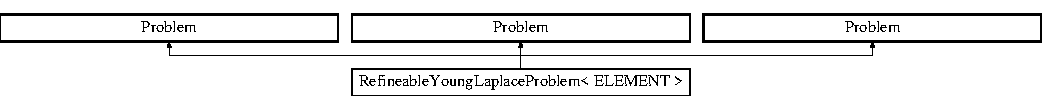
\includegraphics[height=1.287356cm]{classRefineableYoungLaplaceProblem}
\end{center}
\end{figure}
\subsection*{Public Member Functions}
\begin{DoxyCompactItemize}
\item 
\hyperlink{classRefineableYoungLaplaceProblem_a78f77a299f2770a82378fcccf86a0b71}{Refineable\+Young\+Laplace\+Problem} ()
\begin{DoxyCompactList}\small\item\em Constructor\+: \end{DoxyCompactList}\item 
\hyperlink{classRefineableYoungLaplaceProblem_a24b45d5ecdd1d7dbb678e7f74777bf41}{$\sim$\+Refineable\+Young\+Laplace\+Problem} ()
\begin{DoxyCompactList}\small\item\em Destructor (empty) \end{DoxyCompactList}\item 
void \hyperlink{classRefineableYoungLaplaceProblem_a2807bb8cddbfa553df9f5dd170c8645d}{actions\+\_\+before\+\_\+newton\+\_\+solve} ()
\begin{DoxyCompactList}\small\item\em Update the problem specs before solve\+: Empty. \end{DoxyCompactList}\item 
void \hyperlink{classRefineableYoungLaplaceProblem_a0791c90a16016372e09faf3f5721ecbe}{actions\+\_\+after\+\_\+newton\+\_\+solve} ()
\begin{DoxyCompactList}\small\item\em Update the problem after solve\+: Empty. \end{DoxyCompactList}\item 
void \hyperlink{classRefineableYoungLaplaceProblem_ab64eb0b58beb3bb096ecc81b1a3f8a4f}{actions\+\_\+before\+\_\+adapt} ()
\begin{DoxyCompactList}\small\item\em Actions before adapt\+: Wipe the mesh of contact angle elements. \end{DoxyCompactList}\item 
void \hyperlink{classRefineableYoungLaplaceProblem_aa2eab8da1b83091df804ede7c60fac87}{actions\+\_\+after\+\_\+adapt} ()
\begin{DoxyCompactList}\small\item\em Actions after adapt\+: Rebuild the mesh of contact angle elements. \end{DoxyCompactList}\item 
void \hyperlink{classRefineableYoungLaplaceProblem_a4ec7313c8e4015b0c2af0bbef789e70f}{doc\+\_\+solution} (Doc\+Info \&doc\+\_\+info, ofstream \&trace\+\_\+file)
\begin{DoxyCompactList}\small\item\em Doc the solution. Doc\+Info object stores flags/labels for where the output gets written to and the trace file. \end{DoxyCompactList}\item 
\hyperlink{classRefineableYoungLaplaceProblem_a78f77a299f2770a82378fcccf86a0b71}{Refineable\+Young\+Laplace\+Problem} ()
\begin{DoxyCompactList}\small\item\em Constructor\+: \end{DoxyCompactList}\item 
\hyperlink{classRefineableYoungLaplaceProblem_a24b45d5ecdd1d7dbb678e7f74777bf41}{$\sim$\+Refineable\+Young\+Laplace\+Problem} ()
\begin{DoxyCompactList}\small\item\em Destructor (empty) \end{DoxyCompactList}\item 
void \hyperlink{classRefineableYoungLaplaceProblem_a2807bb8cddbfa553df9f5dd170c8645d}{actions\+\_\+before\+\_\+newton\+\_\+solve} ()
\begin{DoxyCompactList}\small\item\em Update the problem specs before solve\+: Empty. \end{DoxyCompactList}\item 
void \hyperlink{classRefineableYoungLaplaceProblem_a0791c90a16016372e09faf3f5721ecbe}{actions\+\_\+after\+\_\+newton\+\_\+solve} ()
\begin{DoxyCompactList}\small\item\em Update the problem after solve\+: Empty. \end{DoxyCompactList}\item 
void \hyperlink{classRefineableYoungLaplaceProblem_ab64eb0b58beb3bb096ecc81b1a3f8a4f}{actions\+\_\+before\+\_\+adapt} ()
\begin{DoxyCompactList}\small\item\em Actions before adapt\+: Wipe the mesh of contact angle elements. \end{DoxyCompactList}\item 
void \hyperlink{classRefineableYoungLaplaceProblem_aa2eab8da1b83091df804ede7c60fac87}{actions\+\_\+after\+\_\+adapt} ()
\begin{DoxyCompactList}\small\item\em Actions after adapt\+: Rebuild the mesh of contact angle elements. \end{DoxyCompactList}\item 
void \hyperlink{classRefineableYoungLaplaceProblem_ac8da9e38012994438200b53d398ce465}{increment\+\_\+parameters} ()
\begin{DoxyCompactList}\small\item\em Increase the problem parameters before each solve. \end{DoxyCompactList}\item 
void \hyperlink{classRefineableYoungLaplaceProblem_a4ec7313c8e4015b0c2af0bbef789e70f}{doc\+\_\+solution} (Doc\+Info \&doc\+\_\+info, ofstream \&trace\+\_\+file)
\begin{DoxyCompactList}\small\item\em Doc the solution. Doc\+Info object stores flags/labels for where the output gets written to and the trace file. \end{DoxyCompactList}\item 
\hyperlink{classRefineableYoungLaplaceProblem_a78f77a299f2770a82378fcccf86a0b71}{Refineable\+Young\+Laplace\+Problem} ()
\begin{DoxyCompactList}\small\item\em Constructor\+: \end{DoxyCompactList}\item 
\hyperlink{classRefineableYoungLaplaceProblem_a24b45d5ecdd1d7dbb678e7f74777bf41}{$\sim$\+Refineable\+Young\+Laplace\+Problem} ()
\begin{DoxyCompactList}\small\item\em Destructor (empty) \end{DoxyCompactList}\item 
void \hyperlink{classRefineableYoungLaplaceProblem_af2a639c1cdfd6334c9023c6bfbe69c8a}{actions\+\_\+before\+\_\+solve} ()
\begin{DoxyCompactList}\small\item\em Update the problem specs before solve\+: Empty. \end{DoxyCompactList}\item 
void \hyperlink{classRefineableYoungLaplaceProblem_a5c472ae3361af18979085c824a47ab53}{actions\+\_\+after\+\_\+solve} ()
\begin{DoxyCompactList}\small\item\em Update the problem after solve\+: Empty. \end{DoxyCompactList}\item 
void \hyperlink{classRefineableYoungLaplaceProblem_ac8da9e38012994438200b53d398ce465}{increment\+\_\+parameters} ()
\begin{DoxyCompactList}\small\item\em Increment problem parameters. \end{DoxyCompactList}\item 
void \hyperlink{classRefineableYoungLaplaceProblem_a4ec7313c8e4015b0c2af0bbef789e70f}{doc\+\_\+solution} (Doc\+Info \&doc\+\_\+info, ofstream \&trace\+\_\+file)
\begin{DoxyCompactList}\small\item\em Doc the solution. Doc\+Info object stores flags/labels for where the output gets written to and the trace file. \end{DoxyCompactList}\end{DoxyCompactItemize}
\subsection*{Private Member Functions}
\begin{DoxyCompactItemize}
\item 
void \hyperlink{classRefineableYoungLaplaceProblem_a00d1304e030120e76d9f316dd4053116}{create\+\_\+contact\+\_\+angle\+\_\+elements} (const unsigned \&b)
\begin{DoxyCompactList}\small\item\em Create Young\+Laplace contact angle elements on the b-\/th boundary of the bulk mesh and add them to contact angle mesh. \end{DoxyCompactList}\item 
void \hyperlink{classRefineableYoungLaplaceProblem_aaa270ba8da395897a5a99d052f076e0c}{delete\+\_\+contact\+\_\+angle\+\_\+elements} ()
\begin{DoxyCompactList}\small\item\em Delete contact angle elements. \end{DoxyCompactList}\item 
void \hyperlink{classRefineableYoungLaplaceProblem_a00d1304e030120e76d9f316dd4053116}{create\+\_\+contact\+\_\+angle\+\_\+elements} (const unsigned \&b)
\begin{DoxyCompactList}\small\item\em Create Young\+Laplace contact angle elements on the b-\/th boundary of the bulk mesh and add them to contact angle mesh. \end{DoxyCompactList}\item 
void \hyperlink{classRefineableYoungLaplaceProblem_aaa270ba8da395897a5a99d052f076e0c}{delete\+\_\+contact\+\_\+angle\+\_\+elements} ()
\begin{DoxyCompactList}\small\item\em Delete contact angle elements. \end{DoxyCompactList}\end{DoxyCompactItemize}
\subsection*{Private Attributes}
\begin{DoxyCompactItemize}
\item 
Refineable\+Rectangular\+Quad\+Mesh$<$ E\+L\+E\+M\+E\+NT $>$ $\ast$ \hyperlink{classRefineableYoungLaplaceProblem_a251d9473d70dea7bfb36d9f0b4bb412d}{Bulk\+\_\+mesh\+\_\+pt}
\begin{DoxyCompactList}\small\item\em Pointer to the \char`\"{}bulk\char`\"{} mesh. \end{DoxyCompactList}\item 
Mesh $\ast$ \hyperlink{classRefineableYoungLaplaceProblem_a36f5dc0f7071ac15fd63c7c477f77fb0}{Contact\+\_\+angle\+\_\+mesh\+\_\+pt}
\begin{DoxyCompactList}\small\item\em Pointer to the contact angle mesh. \end{DoxyCompactList}\item 
Mesh $\ast$ \hyperlink{classRefineableYoungLaplaceProblem_ae2ae72b9b685c052b6a86892f64c2d85}{Height\+\_\+control\+\_\+mesh\+\_\+pt}
\begin{DoxyCompactList}\small\item\em Pointer to mesh containing the height control element. \end{DoxyCompactList}\item 
Node $\ast$ \hyperlink{classRefineableYoungLaplaceProblem_af14d838e5d4a1b9df2595bb08fa5e99d}{Control\+\_\+node\+\_\+pt}
\begin{DoxyCompactList}\small\item\em Node at which the height (displacement along spine) is controlled/doced. \end{DoxyCompactList}\item 
Data $\ast$ \hyperlink{classRefineableYoungLaplaceProblem_a0d667f8f0c41048740c5344619e27584}{Kappa\+\_\+pt}
\begin{DoxyCompactList}\small\item\em Pointer to Data object that stores the prescribed curvature. \end{DoxyCompactList}\item 
Height\+Control\+Element $\ast$ \hyperlink{classRefineableYoungLaplaceProblem_ab97cbf6dc6490194591b03c45642e147}{Height\+\_\+control\+\_\+element\+\_\+pt}
\begin{DoxyCompactList}\small\item\em Pointer to height control element. \end{DoxyCompactList}\item 
Geom\+Object $\ast$ \hyperlink{classRefineableYoungLaplaceProblem_a6092f98c7ffbcd158c783d372d375759}{Boundary\+\_\+pt}
\begin{DoxyCompactList}\small\item\em Pointer to Geom\+Object that specifies the domain bondary. \end{DoxyCompactList}\item 
Refineable\+Quarter\+Circle\+Sector\+Mesh$<$ E\+L\+E\+M\+E\+NT $>$ $\ast$ \hyperlink{classRefineableYoungLaplaceProblem_ab036ff8d3bf66d3f3bb9e977bc6822d3}{Bulk\+\_\+mesh\+\_\+pt}
\begin{DoxyCompactList}\small\item\em Pointer to the \char`\"{}bulk\char`\"{} mesh. \end{DoxyCompactList}\end{DoxyCompactItemize}


\subsection{Detailed Description}
\subsubsection*{template$<$class E\+L\+E\+M\+E\+NT$>$\newline
class Refineable\+Young\+Laplace\+Problem$<$ E\+L\+E\+M\+E\+N\+T $>$}

2D Refineable\+Young\+Laplace problem on rectangular domain, discretised with 2D Q\+Refineable\+Young\+Laplace elements. The specific type of element is specified via the template parameter.

2D Refineable\+Young\+Laplace problem on a circle sector, discretised with 2D Q\+Refineable\+Young\+Laplace elements. The specific type of element is specified via the template parameter. 

Definition at line 142 of file refineable\+\_\+t\+\_\+junction.\+cc.



\subsection{Constructor \& Destructor Documentation}
\mbox{\Hypertarget{classRefineableYoungLaplaceProblem_a78f77a299f2770a82378fcccf86a0b71}\label{classRefineableYoungLaplaceProblem_a78f77a299f2770a82378fcccf86a0b71}} 
\index{Refineable\+Young\+Laplace\+Problem@{Refineable\+Young\+Laplace\+Problem}!Refineable\+Young\+Laplace\+Problem@{Refineable\+Young\+Laplace\+Problem}}
\index{Refineable\+Young\+Laplace\+Problem@{Refineable\+Young\+Laplace\+Problem}!Refineable\+Young\+Laplace\+Problem@{Refineable\+Young\+Laplace\+Problem}}
\subsubsection{\texorpdfstring{Refineable\+Young\+Laplace\+Problem()}{RefineableYoungLaplaceProblem()}\hspace{0.1cm}{\footnotesize\ttfamily [1/3]}}
{\footnotesize\ttfamily template$<$class E\+L\+E\+M\+E\+NT $>$ \\
\hyperlink{classRefineableYoungLaplaceProblem}{Refineable\+Young\+Laplace\+Problem}$<$ E\+L\+E\+M\+E\+NT $>$\+::\hyperlink{classRefineableYoungLaplaceProblem}{Refineable\+Young\+Laplace\+Problem} (\begin{DoxyParamCaption}{ }\end{DoxyParamCaption})}



Constructor\+: 

Constructor for Refineable\+Young\+Laplace problem. 

Definition at line 230 of file refineable\+\_\+t\+\_\+junction.\+cc.



References Global\+Parameters\+::\+Controlled\+\_\+height, Global\+Parameters\+::\+Cos\+\_\+gamma, Global\+Parameters\+::\+Kappa\+\_\+pt, Global\+Parameters\+::\+L\+\_\+x, Global\+Parameters\+::\+L\+\_\+y, Global\+Parameters\+::spine\+\_\+base\+\_\+function(), and Global\+Parameters\+::spine\+\_\+function().

\mbox{\Hypertarget{classRefineableYoungLaplaceProblem_a24b45d5ecdd1d7dbb678e7f74777bf41}\label{classRefineableYoungLaplaceProblem_a24b45d5ecdd1d7dbb678e7f74777bf41}} 
\index{Refineable\+Young\+Laplace\+Problem@{Refineable\+Young\+Laplace\+Problem}!````~Refineable\+Young\+Laplace\+Problem@{$\sim$\+Refineable\+Young\+Laplace\+Problem}}
\index{````~Refineable\+Young\+Laplace\+Problem@{$\sim$\+Refineable\+Young\+Laplace\+Problem}!Refineable\+Young\+Laplace\+Problem@{Refineable\+Young\+Laplace\+Problem}}
\subsubsection{\texorpdfstring{$\sim$\+Refineable\+Young\+Laplace\+Problem()}{~RefineableYoungLaplaceProblem()}\hspace{0.1cm}{\footnotesize\ttfamily [1/3]}}
{\footnotesize\ttfamily template$<$class E\+L\+E\+M\+E\+NT$>$ \\
\hyperlink{classRefineableYoungLaplaceProblem}{Refineable\+Young\+Laplace\+Problem}$<$ E\+L\+E\+M\+E\+NT $>$\+::$\sim$\hyperlink{classRefineableYoungLaplaceProblem}{Refineable\+Young\+Laplace\+Problem} (\begin{DoxyParamCaption}{ }\end{DoxyParamCaption})\hspace{0.3cm}{\ttfamily [inline]}}



Destructor (empty) 



Definition at line 151 of file refineable\+\_\+t\+\_\+junction.\+cc.

\mbox{\Hypertarget{classRefineableYoungLaplaceProblem_a78f77a299f2770a82378fcccf86a0b71}\label{classRefineableYoungLaplaceProblem_a78f77a299f2770a82378fcccf86a0b71}} 
\index{Refineable\+Young\+Laplace\+Problem@{Refineable\+Young\+Laplace\+Problem}!Refineable\+Young\+Laplace\+Problem@{Refineable\+Young\+Laplace\+Problem}}
\index{Refineable\+Young\+Laplace\+Problem@{Refineable\+Young\+Laplace\+Problem}!Refineable\+Young\+Laplace\+Problem@{Refineable\+Young\+Laplace\+Problem}}
\subsubsection{\texorpdfstring{Refineable\+Young\+Laplace\+Problem()}{RefineableYoungLaplaceProblem()}\hspace{0.1cm}{\footnotesize\ttfamily [2/3]}}
{\footnotesize\ttfamily template$<$class E\+L\+E\+M\+E\+NT$>$ \\
\hyperlink{classRefineableYoungLaplaceProblem}{Refineable\+Young\+Laplace\+Problem}$<$ E\+L\+E\+M\+E\+NT $>$\+::\hyperlink{classRefineableYoungLaplaceProblem}{Refineable\+Young\+Laplace\+Problem} (\begin{DoxyParamCaption}{ }\end{DoxyParamCaption})}



Constructor\+: 

\mbox{\Hypertarget{classRefineableYoungLaplaceProblem_a24b45d5ecdd1d7dbb678e7f74777bf41}\label{classRefineableYoungLaplaceProblem_a24b45d5ecdd1d7dbb678e7f74777bf41}} 
\index{Refineable\+Young\+Laplace\+Problem@{Refineable\+Young\+Laplace\+Problem}!````~Refineable\+Young\+Laplace\+Problem@{$\sim$\+Refineable\+Young\+Laplace\+Problem}}
\index{````~Refineable\+Young\+Laplace\+Problem@{$\sim$\+Refineable\+Young\+Laplace\+Problem}!Refineable\+Young\+Laplace\+Problem@{Refineable\+Young\+Laplace\+Problem}}
\subsubsection{\texorpdfstring{$\sim$\+Refineable\+Young\+Laplace\+Problem()}{~RefineableYoungLaplaceProblem()}\hspace{0.1cm}{\footnotesize\ttfamily [2/3]}}
{\footnotesize\ttfamily template$<$class E\+L\+E\+M\+E\+NT$>$ \\
\hyperlink{classRefineableYoungLaplaceProblem}{Refineable\+Young\+Laplace\+Problem}$<$ E\+L\+E\+M\+E\+NT $>$\+::$\sim$\hyperlink{classRefineableYoungLaplaceProblem}{Refineable\+Young\+Laplace\+Problem} (\begin{DoxyParamCaption}{ }\end{DoxyParamCaption})\hspace{0.3cm}{\ttfamily [inline]}}



Destructor (empty) 



Definition at line 63 of file refineable\+\_\+young\+\_\+laplace.\+cc.

\mbox{\Hypertarget{classRefineableYoungLaplaceProblem_a78f77a299f2770a82378fcccf86a0b71}\label{classRefineableYoungLaplaceProblem_a78f77a299f2770a82378fcccf86a0b71}} 
\index{Refineable\+Young\+Laplace\+Problem@{Refineable\+Young\+Laplace\+Problem}!Refineable\+Young\+Laplace\+Problem@{Refineable\+Young\+Laplace\+Problem}}
\index{Refineable\+Young\+Laplace\+Problem@{Refineable\+Young\+Laplace\+Problem}!Refineable\+Young\+Laplace\+Problem@{Refineable\+Young\+Laplace\+Problem}}
\subsubsection{\texorpdfstring{Refineable\+Young\+Laplace\+Problem()}{RefineableYoungLaplaceProblem()}\hspace{0.1cm}{\footnotesize\ttfamily [3/3]}}
{\footnotesize\ttfamily template$<$class E\+L\+E\+M\+E\+NT$>$ \\
\hyperlink{classRefineableYoungLaplaceProblem}{Refineable\+Young\+Laplace\+Problem}$<$ E\+L\+E\+M\+E\+NT $>$\+::\hyperlink{classRefineableYoungLaplaceProblem}{Refineable\+Young\+Laplace\+Problem} (\begin{DoxyParamCaption}{ }\end{DoxyParamCaption})}



Constructor\+: 

\mbox{\Hypertarget{classRefineableYoungLaplaceProblem_a24b45d5ecdd1d7dbb678e7f74777bf41}\label{classRefineableYoungLaplaceProblem_a24b45d5ecdd1d7dbb678e7f74777bf41}} 
\index{Refineable\+Young\+Laplace\+Problem@{Refineable\+Young\+Laplace\+Problem}!````~Refineable\+Young\+Laplace\+Problem@{$\sim$\+Refineable\+Young\+Laplace\+Problem}}
\index{````~Refineable\+Young\+Laplace\+Problem@{$\sim$\+Refineable\+Young\+Laplace\+Problem}!Refineable\+Young\+Laplace\+Problem@{Refineable\+Young\+Laplace\+Problem}}
\subsubsection{\texorpdfstring{$\sim$\+Refineable\+Young\+Laplace\+Problem()}{~RefineableYoungLaplaceProblem()}\hspace{0.1cm}{\footnotesize\ttfamily [3/3]}}
{\footnotesize\ttfamily template$<$class E\+L\+E\+M\+E\+NT$>$ \\
\hyperlink{classRefineableYoungLaplaceProblem}{Refineable\+Young\+Laplace\+Problem}$<$ E\+L\+E\+M\+E\+NT $>$\+::$\sim$\hyperlink{classRefineableYoungLaplaceProblem}{Refineable\+Young\+Laplace\+Problem} (\begin{DoxyParamCaption}{ }\end{DoxyParamCaption})\hspace{0.3cm}{\ttfamily [inline]}}



Destructor (empty) 



Definition at line 66 of file spherical\+\_\+cap\+\_\+in\+\_\+cylinder.\+cc.



\subsection{Member Function Documentation}
\mbox{\Hypertarget{classRefineableYoungLaplaceProblem_aa2eab8da1b83091df804ede7c60fac87}\label{classRefineableYoungLaplaceProblem_aa2eab8da1b83091df804ede7c60fac87}} 
\index{Refineable\+Young\+Laplace\+Problem@{Refineable\+Young\+Laplace\+Problem}!actions\+\_\+after\+\_\+adapt@{actions\+\_\+after\+\_\+adapt}}
\index{actions\+\_\+after\+\_\+adapt@{actions\+\_\+after\+\_\+adapt}!Refineable\+Young\+Laplace\+Problem@{Refineable\+Young\+Laplace\+Problem}}
\subsubsection{\texorpdfstring{actions\+\_\+after\+\_\+adapt()}{actions\_after\_adapt()}\hspace{0.1cm}{\footnotesize\ttfamily [1/2]}}
{\footnotesize\ttfamily template$<$class E\+L\+E\+M\+E\+NT$>$ \\
void \hyperlink{classRefineableYoungLaplaceProblem}{Refineable\+Young\+Laplace\+Problem}$<$ E\+L\+E\+M\+E\+NT $>$\+::actions\+\_\+after\+\_\+adapt (\begin{DoxyParamCaption}{ }\end{DoxyParamCaption})\hspace{0.3cm}{\ttfamily [inline]}}



Actions after adapt\+: Rebuild the mesh of contact angle elements. 



Definition at line 83 of file refineable\+\_\+young\+\_\+laplace.\+cc.



References Global\+Parameters\+::\+Case, Global\+Parameters\+::\+Cos\+\_\+gamma, and Global\+Parameters\+::\+T\+\_\+junction\+\_\+with\+\_\+nonzero\+\_\+contact\+\_\+angle.

\mbox{\Hypertarget{classRefineableYoungLaplaceProblem_aa2eab8da1b83091df804ede7c60fac87}\label{classRefineableYoungLaplaceProblem_aa2eab8da1b83091df804ede7c60fac87}} 
\index{Refineable\+Young\+Laplace\+Problem@{Refineable\+Young\+Laplace\+Problem}!actions\+\_\+after\+\_\+adapt@{actions\+\_\+after\+\_\+adapt}}
\index{actions\+\_\+after\+\_\+adapt@{actions\+\_\+after\+\_\+adapt}!Refineable\+Young\+Laplace\+Problem@{Refineable\+Young\+Laplace\+Problem}}
\subsubsection{\texorpdfstring{actions\+\_\+after\+\_\+adapt()}{actions\_after\_adapt()}\hspace{0.1cm}{\footnotesize\ttfamily [2/2]}}
{\footnotesize\ttfamily template$<$class E\+L\+E\+M\+E\+NT$>$ \\
void \hyperlink{classRefineableYoungLaplaceProblem}{Refineable\+Young\+Laplace\+Problem}$<$ E\+L\+E\+M\+E\+NT $>$\+::actions\+\_\+after\+\_\+adapt (\begin{DoxyParamCaption}{ }\end{DoxyParamCaption})\hspace{0.3cm}{\ttfamily [inline]}}



Actions after adapt\+: Rebuild the mesh of contact angle elements. 



Definition at line 171 of file refineable\+\_\+t\+\_\+junction.\+cc.



References Global\+Parameters\+::\+Cos\+\_\+gamma.

\mbox{\Hypertarget{classRefineableYoungLaplaceProblem_a0791c90a16016372e09faf3f5721ecbe}\label{classRefineableYoungLaplaceProblem_a0791c90a16016372e09faf3f5721ecbe}} 
\index{Refineable\+Young\+Laplace\+Problem@{Refineable\+Young\+Laplace\+Problem}!actions\+\_\+after\+\_\+newton\+\_\+solve@{actions\+\_\+after\+\_\+newton\+\_\+solve}}
\index{actions\+\_\+after\+\_\+newton\+\_\+solve@{actions\+\_\+after\+\_\+newton\+\_\+solve}!Refineable\+Young\+Laplace\+Problem@{Refineable\+Young\+Laplace\+Problem}}
\subsubsection{\texorpdfstring{actions\+\_\+after\+\_\+newton\+\_\+solve()}{actions\_after\_newton\_solve()}\hspace{0.1cm}{\footnotesize\ttfamily [1/2]}}
{\footnotesize\ttfamily template$<$class E\+L\+E\+M\+E\+NT$>$ \\
void \hyperlink{classRefineableYoungLaplaceProblem}{Refineable\+Young\+Laplace\+Problem}$<$ E\+L\+E\+M\+E\+NT $>$\+::actions\+\_\+after\+\_\+newton\+\_\+solve (\begin{DoxyParamCaption}{ }\end{DoxyParamCaption})\hspace{0.3cm}{\ttfamily [inline]}}



Update the problem after solve\+: Empty. 



Definition at line 69 of file refineable\+\_\+young\+\_\+laplace.\+cc.

\mbox{\Hypertarget{classRefineableYoungLaplaceProblem_a0791c90a16016372e09faf3f5721ecbe}\label{classRefineableYoungLaplaceProblem_a0791c90a16016372e09faf3f5721ecbe}} 
\index{Refineable\+Young\+Laplace\+Problem@{Refineable\+Young\+Laplace\+Problem}!actions\+\_\+after\+\_\+newton\+\_\+solve@{actions\+\_\+after\+\_\+newton\+\_\+solve}}
\index{actions\+\_\+after\+\_\+newton\+\_\+solve@{actions\+\_\+after\+\_\+newton\+\_\+solve}!Refineable\+Young\+Laplace\+Problem@{Refineable\+Young\+Laplace\+Problem}}
\subsubsection{\texorpdfstring{actions\+\_\+after\+\_\+newton\+\_\+solve()}{actions\_after\_newton\_solve()}\hspace{0.1cm}{\footnotesize\ttfamily [2/2]}}
{\footnotesize\ttfamily template$<$class E\+L\+E\+M\+E\+NT$>$ \\
void \hyperlink{classRefineableYoungLaplaceProblem}{Refineable\+Young\+Laplace\+Problem}$<$ E\+L\+E\+M\+E\+NT $>$\+::actions\+\_\+after\+\_\+newton\+\_\+solve (\begin{DoxyParamCaption}{ }\end{DoxyParamCaption})\hspace{0.3cm}{\ttfamily [inline]}}



Update the problem after solve\+: Empty. 



Definition at line 157 of file refineable\+\_\+t\+\_\+junction.\+cc.

\mbox{\Hypertarget{classRefineableYoungLaplaceProblem_a5c472ae3361af18979085c824a47ab53}\label{classRefineableYoungLaplaceProblem_a5c472ae3361af18979085c824a47ab53}} 
\index{Refineable\+Young\+Laplace\+Problem@{Refineable\+Young\+Laplace\+Problem}!actions\+\_\+after\+\_\+solve@{actions\+\_\+after\+\_\+solve}}
\index{actions\+\_\+after\+\_\+solve@{actions\+\_\+after\+\_\+solve}!Refineable\+Young\+Laplace\+Problem@{Refineable\+Young\+Laplace\+Problem}}
\subsubsection{\texorpdfstring{actions\+\_\+after\+\_\+solve()}{actions\_after\_solve()}}
{\footnotesize\ttfamily template$<$class E\+L\+E\+M\+E\+NT$>$ \\
void \hyperlink{classRefineableYoungLaplaceProblem}{Refineable\+Young\+Laplace\+Problem}$<$ E\+L\+E\+M\+E\+NT $>$\+::actions\+\_\+after\+\_\+solve (\begin{DoxyParamCaption}{ }\end{DoxyParamCaption})\hspace{0.3cm}{\ttfamily [inline]}}



Update the problem after solve\+: Empty. 



Definition at line 72 of file spherical\+\_\+cap\+\_\+in\+\_\+cylinder.\+cc.

\mbox{\Hypertarget{classRefineableYoungLaplaceProblem_ab64eb0b58beb3bb096ecc81b1a3f8a4f}\label{classRefineableYoungLaplaceProblem_ab64eb0b58beb3bb096ecc81b1a3f8a4f}} 
\index{Refineable\+Young\+Laplace\+Problem@{Refineable\+Young\+Laplace\+Problem}!actions\+\_\+before\+\_\+adapt@{actions\+\_\+before\+\_\+adapt}}
\index{actions\+\_\+before\+\_\+adapt@{actions\+\_\+before\+\_\+adapt}!Refineable\+Young\+Laplace\+Problem@{Refineable\+Young\+Laplace\+Problem}}
\subsubsection{\texorpdfstring{actions\+\_\+before\+\_\+adapt()}{actions\_before\_adapt()}\hspace{0.1cm}{\footnotesize\ttfamily [1/2]}}
{\footnotesize\ttfamily template$<$class E\+L\+E\+M\+E\+NT$>$ \\
void \hyperlink{classRefineableYoungLaplaceProblem}{Refineable\+Young\+Laplace\+Problem}$<$ E\+L\+E\+M\+E\+NT $>$\+::actions\+\_\+before\+\_\+adapt (\begin{DoxyParamCaption}{ }\end{DoxyParamCaption})\hspace{0.3cm}{\ttfamily [inline]}}



Actions before adapt\+: Wipe the mesh of contact angle elements. 



Definition at line 72 of file refineable\+\_\+young\+\_\+laplace.\+cc.

\mbox{\Hypertarget{classRefineableYoungLaplaceProblem_ab64eb0b58beb3bb096ecc81b1a3f8a4f}\label{classRefineableYoungLaplaceProblem_ab64eb0b58beb3bb096ecc81b1a3f8a4f}} 
\index{Refineable\+Young\+Laplace\+Problem@{Refineable\+Young\+Laplace\+Problem}!actions\+\_\+before\+\_\+adapt@{actions\+\_\+before\+\_\+adapt}}
\index{actions\+\_\+before\+\_\+adapt@{actions\+\_\+before\+\_\+adapt}!Refineable\+Young\+Laplace\+Problem@{Refineable\+Young\+Laplace\+Problem}}
\subsubsection{\texorpdfstring{actions\+\_\+before\+\_\+adapt()}{actions\_before\_adapt()}\hspace{0.1cm}{\footnotesize\ttfamily [2/2]}}
{\footnotesize\ttfamily template$<$class E\+L\+E\+M\+E\+NT$>$ \\
void \hyperlink{classRefineableYoungLaplaceProblem}{Refineable\+Young\+Laplace\+Problem}$<$ E\+L\+E\+M\+E\+NT $>$\+::actions\+\_\+before\+\_\+adapt (\begin{DoxyParamCaption}{ }\end{DoxyParamCaption})\hspace{0.3cm}{\ttfamily [inline]}}



Actions before adapt\+: Wipe the mesh of contact angle elements. 



Definition at line 160 of file refineable\+\_\+t\+\_\+junction.\+cc.

\mbox{\Hypertarget{classRefineableYoungLaplaceProblem_a2807bb8cddbfa553df9f5dd170c8645d}\label{classRefineableYoungLaplaceProblem_a2807bb8cddbfa553df9f5dd170c8645d}} 
\index{Refineable\+Young\+Laplace\+Problem@{Refineable\+Young\+Laplace\+Problem}!actions\+\_\+before\+\_\+newton\+\_\+solve@{actions\+\_\+before\+\_\+newton\+\_\+solve}}
\index{actions\+\_\+before\+\_\+newton\+\_\+solve@{actions\+\_\+before\+\_\+newton\+\_\+solve}!Refineable\+Young\+Laplace\+Problem@{Refineable\+Young\+Laplace\+Problem}}
\subsubsection{\texorpdfstring{actions\+\_\+before\+\_\+newton\+\_\+solve()}{actions\_before\_newton\_solve()}\hspace{0.1cm}{\footnotesize\ttfamily [1/2]}}
{\footnotesize\ttfamily template$<$class E\+L\+E\+M\+E\+NT$>$ \\
void \hyperlink{classRefineableYoungLaplaceProblem}{Refineable\+Young\+Laplace\+Problem}$<$ E\+L\+E\+M\+E\+NT $>$\+::actions\+\_\+before\+\_\+newton\+\_\+solve (\begin{DoxyParamCaption}{ }\end{DoxyParamCaption})\hspace{0.3cm}{\ttfamily [inline]}}



Update the problem specs before solve\+: Empty. 



Definition at line 66 of file refineable\+\_\+young\+\_\+laplace.\+cc.

\mbox{\Hypertarget{classRefineableYoungLaplaceProblem_a2807bb8cddbfa553df9f5dd170c8645d}\label{classRefineableYoungLaplaceProblem_a2807bb8cddbfa553df9f5dd170c8645d}} 
\index{Refineable\+Young\+Laplace\+Problem@{Refineable\+Young\+Laplace\+Problem}!actions\+\_\+before\+\_\+newton\+\_\+solve@{actions\+\_\+before\+\_\+newton\+\_\+solve}}
\index{actions\+\_\+before\+\_\+newton\+\_\+solve@{actions\+\_\+before\+\_\+newton\+\_\+solve}!Refineable\+Young\+Laplace\+Problem@{Refineable\+Young\+Laplace\+Problem}}
\subsubsection{\texorpdfstring{actions\+\_\+before\+\_\+newton\+\_\+solve()}{actions\_before\_newton\_solve()}\hspace{0.1cm}{\footnotesize\ttfamily [2/2]}}
{\footnotesize\ttfamily template$<$class E\+L\+E\+M\+E\+NT$>$ \\
void \hyperlink{classRefineableYoungLaplaceProblem}{Refineable\+Young\+Laplace\+Problem}$<$ E\+L\+E\+M\+E\+NT $>$\+::actions\+\_\+before\+\_\+newton\+\_\+solve (\begin{DoxyParamCaption}{ }\end{DoxyParamCaption})\hspace{0.3cm}{\ttfamily [inline]}}



Update the problem specs before solve\+: Empty. 



Definition at line 154 of file refineable\+\_\+t\+\_\+junction.\+cc.

\mbox{\Hypertarget{classRefineableYoungLaplaceProblem_af2a639c1cdfd6334c9023c6bfbe69c8a}\label{classRefineableYoungLaplaceProblem_af2a639c1cdfd6334c9023c6bfbe69c8a}} 
\index{Refineable\+Young\+Laplace\+Problem@{Refineable\+Young\+Laplace\+Problem}!actions\+\_\+before\+\_\+solve@{actions\+\_\+before\+\_\+solve}}
\index{actions\+\_\+before\+\_\+solve@{actions\+\_\+before\+\_\+solve}!Refineable\+Young\+Laplace\+Problem@{Refineable\+Young\+Laplace\+Problem}}
\subsubsection{\texorpdfstring{actions\+\_\+before\+\_\+solve()}{actions\_before\_solve()}}
{\footnotesize\ttfamily template$<$class E\+L\+E\+M\+E\+NT$>$ \\
void \hyperlink{classRefineableYoungLaplaceProblem}{Refineable\+Young\+Laplace\+Problem}$<$ E\+L\+E\+M\+E\+NT $>$\+::actions\+\_\+before\+\_\+solve (\begin{DoxyParamCaption}{ }\end{DoxyParamCaption})\hspace{0.3cm}{\ttfamily [inline]}}



Update the problem specs before solve\+: Empty. 



Definition at line 69 of file spherical\+\_\+cap\+\_\+in\+\_\+cylinder.\+cc.

\mbox{\Hypertarget{classRefineableYoungLaplaceProblem_a00d1304e030120e76d9f316dd4053116}\label{classRefineableYoungLaplaceProblem_a00d1304e030120e76d9f316dd4053116}} 
\index{Refineable\+Young\+Laplace\+Problem@{Refineable\+Young\+Laplace\+Problem}!create\+\_\+contact\+\_\+angle\+\_\+elements@{create\+\_\+contact\+\_\+angle\+\_\+elements}}
\index{create\+\_\+contact\+\_\+angle\+\_\+elements@{create\+\_\+contact\+\_\+angle\+\_\+elements}!Refineable\+Young\+Laplace\+Problem@{Refineable\+Young\+Laplace\+Problem}}
\subsubsection{\texorpdfstring{create\+\_\+contact\+\_\+angle\+\_\+elements()}{create\_contact\_angle\_elements()}\hspace{0.1cm}{\footnotesize\ttfamily [1/2]}}
{\footnotesize\ttfamily template$<$class E\+L\+E\+M\+E\+NT$>$ \\
void \hyperlink{classRefineableYoungLaplaceProblem}{Refineable\+Young\+Laplace\+Problem}$<$ E\+L\+E\+M\+E\+NT $>$\+::create\+\_\+contact\+\_\+angle\+\_\+elements (\begin{DoxyParamCaption}\item[{const unsigned \&}]{b }\end{DoxyParamCaption})\hspace{0.3cm}{\ttfamily [private]}}



Create Young\+Laplace contact angle elements on the b-\/th boundary of the bulk mesh and add them to contact angle mesh. 

\mbox{\Hypertarget{classRefineableYoungLaplaceProblem_a00d1304e030120e76d9f316dd4053116}\label{classRefineableYoungLaplaceProblem_a00d1304e030120e76d9f316dd4053116}} 
\index{Refineable\+Young\+Laplace\+Problem@{Refineable\+Young\+Laplace\+Problem}!create\+\_\+contact\+\_\+angle\+\_\+elements@{create\+\_\+contact\+\_\+angle\+\_\+elements}}
\index{create\+\_\+contact\+\_\+angle\+\_\+elements@{create\+\_\+contact\+\_\+angle\+\_\+elements}!Refineable\+Young\+Laplace\+Problem@{Refineable\+Young\+Laplace\+Problem}}
\subsubsection{\texorpdfstring{create\+\_\+contact\+\_\+angle\+\_\+elements()}{create\_contact\_angle\_elements()}\hspace{0.1cm}{\footnotesize\ttfamily [2/2]}}
{\footnotesize\ttfamily template$<$class E\+L\+E\+M\+E\+NT $>$ \\
void \hyperlink{classRefineableYoungLaplaceProblem}{Refineable\+Young\+Laplace\+Problem}$<$ E\+L\+E\+M\+E\+NT $>$\+::create\+\_\+contact\+\_\+angle\+\_\+elements (\begin{DoxyParamCaption}\item[{const unsigned \&}]{b }\end{DoxyParamCaption})\hspace{0.3cm}{\ttfamily [private]}}



Create Young\+Laplace contact angle elements on the b-\/th boundary of the bulk mesh and add them to contact angle mesh. 

Create Young\+Laplace contact angle elements on the b-\/th boundary of the bulk mesh and add them to the contact angle mesh 

Definition at line 377 of file refineable\+\_\+t\+\_\+junction.\+cc.

\mbox{\Hypertarget{classRefineableYoungLaplaceProblem_aaa270ba8da395897a5a99d052f076e0c}\label{classRefineableYoungLaplaceProblem_aaa270ba8da395897a5a99d052f076e0c}} 
\index{Refineable\+Young\+Laplace\+Problem@{Refineable\+Young\+Laplace\+Problem}!delete\+\_\+contact\+\_\+angle\+\_\+elements@{delete\+\_\+contact\+\_\+angle\+\_\+elements}}
\index{delete\+\_\+contact\+\_\+angle\+\_\+elements@{delete\+\_\+contact\+\_\+angle\+\_\+elements}!Refineable\+Young\+Laplace\+Problem@{Refineable\+Young\+Laplace\+Problem}}
\subsubsection{\texorpdfstring{delete\+\_\+contact\+\_\+angle\+\_\+elements()}{delete\_contact\_angle\_elements()}\hspace{0.1cm}{\footnotesize\ttfamily [1/2]}}
{\footnotesize\ttfamily template$<$class E\+L\+E\+M\+E\+NT$>$ \\
void \hyperlink{classRefineableYoungLaplaceProblem}{Refineable\+Young\+Laplace\+Problem}$<$ E\+L\+E\+M\+E\+NT $>$\+::delete\+\_\+contact\+\_\+angle\+\_\+elements (\begin{DoxyParamCaption}{ }\end{DoxyParamCaption})\hspace{0.3cm}{\ttfamily [private]}}



Delete contact angle elements. 

\mbox{\Hypertarget{classRefineableYoungLaplaceProblem_aaa270ba8da395897a5a99d052f076e0c}\label{classRefineableYoungLaplaceProblem_aaa270ba8da395897a5a99d052f076e0c}} 
\index{Refineable\+Young\+Laplace\+Problem@{Refineable\+Young\+Laplace\+Problem}!delete\+\_\+contact\+\_\+angle\+\_\+elements@{delete\+\_\+contact\+\_\+angle\+\_\+elements}}
\index{delete\+\_\+contact\+\_\+angle\+\_\+elements@{delete\+\_\+contact\+\_\+angle\+\_\+elements}!Refineable\+Young\+Laplace\+Problem@{Refineable\+Young\+Laplace\+Problem}}
\subsubsection{\texorpdfstring{delete\+\_\+contact\+\_\+angle\+\_\+elements()}{delete\_contact\_angle\_elements()}\hspace{0.1cm}{\footnotesize\ttfamily [2/2]}}
{\footnotesize\ttfamily template$<$class E\+L\+E\+M\+E\+NT $>$ \\
void \hyperlink{classRefineableYoungLaplaceProblem}{Refineable\+Young\+Laplace\+Problem}$<$ E\+L\+E\+M\+E\+NT $>$\+::delete\+\_\+contact\+\_\+angle\+\_\+elements (\begin{DoxyParamCaption}{ }\end{DoxyParamCaption})\hspace{0.3cm}{\ttfamily [private]}}



Delete contact angle elements. 

Delete Young\+Laplace contact angle elements. 

Definition at line 409 of file refineable\+\_\+t\+\_\+junction.\+cc.

\mbox{\Hypertarget{classRefineableYoungLaplaceProblem_a4ec7313c8e4015b0c2af0bbef789e70f}\label{classRefineableYoungLaplaceProblem_a4ec7313c8e4015b0c2af0bbef789e70f}} 
\index{Refineable\+Young\+Laplace\+Problem@{Refineable\+Young\+Laplace\+Problem}!doc\+\_\+solution@{doc\+\_\+solution}}
\index{doc\+\_\+solution@{doc\+\_\+solution}!Refineable\+Young\+Laplace\+Problem@{Refineable\+Young\+Laplace\+Problem}}
\subsubsection{\texorpdfstring{doc\+\_\+solution()}{doc\_solution()}\hspace{0.1cm}{\footnotesize\ttfamily [1/3]}}
{\footnotesize\ttfamily template$<$class E\+L\+E\+M\+E\+NT$>$ \\
void \hyperlink{classRefineableYoungLaplaceProblem}{Refineable\+Young\+Laplace\+Problem}$<$ E\+L\+E\+M\+E\+NT $>$\+::doc\+\_\+solution (\begin{DoxyParamCaption}\item[{Doc\+Info \&}]{doc\+\_\+info,  }\item[{ofstream \&}]{trace\+\_\+file }\end{DoxyParamCaption})}



Doc the solution. Doc\+Info object stores flags/labels for where the output gets written to and the trace file. 

\mbox{\Hypertarget{classRefineableYoungLaplaceProblem_a4ec7313c8e4015b0c2af0bbef789e70f}\label{classRefineableYoungLaplaceProblem_a4ec7313c8e4015b0c2af0bbef789e70f}} 
\index{Refineable\+Young\+Laplace\+Problem@{Refineable\+Young\+Laplace\+Problem}!doc\+\_\+solution@{doc\+\_\+solution}}
\index{doc\+\_\+solution@{doc\+\_\+solution}!Refineable\+Young\+Laplace\+Problem@{Refineable\+Young\+Laplace\+Problem}}
\subsubsection{\texorpdfstring{doc\+\_\+solution()}{doc\_solution()}\hspace{0.1cm}{\footnotesize\ttfamily [2/3]}}
{\footnotesize\ttfamily template$<$class E\+L\+E\+M\+E\+NT$>$ \\
void \hyperlink{classRefineableYoungLaplaceProblem}{Refineable\+Young\+Laplace\+Problem}$<$ E\+L\+E\+M\+E\+NT $>$\+::doc\+\_\+solution (\begin{DoxyParamCaption}\item[{Doc\+Info \&}]{doc\+\_\+info,  }\item[{ofstream \&}]{trace\+\_\+file }\end{DoxyParamCaption})}



Doc the solution. Doc\+Info object stores flags/labels for where the output gets written to and the trace file. 

\mbox{\Hypertarget{classRefineableYoungLaplaceProblem_a4ec7313c8e4015b0c2af0bbef789e70f}\label{classRefineableYoungLaplaceProblem_a4ec7313c8e4015b0c2af0bbef789e70f}} 
\index{Refineable\+Young\+Laplace\+Problem@{Refineable\+Young\+Laplace\+Problem}!doc\+\_\+solution@{doc\+\_\+solution}}
\index{doc\+\_\+solution@{doc\+\_\+solution}!Refineable\+Young\+Laplace\+Problem@{Refineable\+Young\+Laplace\+Problem}}
\subsubsection{\texorpdfstring{doc\+\_\+solution()}{doc\_solution()}\hspace{0.1cm}{\footnotesize\ttfamily [3/3]}}
{\footnotesize\ttfamily template$<$class E\+L\+E\+M\+E\+NT $>$ \\
void \hyperlink{classRefineableYoungLaplaceProblem}{Refineable\+Young\+Laplace\+Problem}$<$ E\+L\+E\+M\+E\+NT $>$\+::doc\+\_\+solution (\begin{DoxyParamCaption}\item[{Doc\+Info \&}]{doc\+\_\+info,  }\item[{ofstream \&}]{trace\+\_\+file }\end{DoxyParamCaption})}



Doc the solution. Doc\+Info object stores flags/labels for where the output gets written to and the trace file. 

Doc the solution\+: doc\+\_\+info contains labels/output directory etc. 

Definition at line 434 of file refineable\+\_\+t\+\_\+junction.\+cc.



References Global\+Parameters\+::\+Kappa\+\_\+pt.



Referenced by Refineable\+Young\+Laplace\+Problem$<$ E\+L\+E\+M\+E\+N\+T $>$\+::increment\+\_\+parameters(), main(), and run\+\_\+it().

\mbox{\Hypertarget{classRefineableYoungLaplaceProblem_ac8da9e38012994438200b53d398ce465}\label{classRefineableYoungLaplaceProblem_ac8da9e38012994438200b53d398ce465}} 
\index{Refineable\+Young\+Laplace\+Problem@{Refineable\+Young\+Laplace\+Problem}!increment\+\_\+parameters@{increment\+\_\+parameters}}
\index{increment\+\_\+parameters@{increment\+\_\+parameters}!Refineable\+Young\+Laplace\+Problem@{Refineable\+Young\+Laplace\+Problem}}
\subsubsection{\texorpdfstring{increment\+\_\+parameters()}{increment\_parameters()}\hspace{0.1cm}{\footnotesize\ttfamily [1/2]}}
{\footnotesize\ttfamily template$<$class E\+L\+E\+M\+E\+NT$>$ \\
void \hyperlink{classRefineableYoungLaplaceProblem}{Refineable\+Young\+Laplace\+Problem}$<$ E\+L\+E\+M\+E\+NT $>$\+::increment\+\_\+parameters (\begin{DoxyParamCaption}{ }\end{DoxyParamCaption})}



Increment problem parameters. 

\mbox{\Hypertarget{classRefineableYoungLaplaceProblem_ac8da9e38012994438200b53d398ce465}\label{classRefineableYoungLaplaceProblem_ac8da9e38012994438200b53d398ce465}} 
\index{Refineable\+Young\+Laplace\+Problem@{Refineable\+Young\+Laplace\+Problem}!increment\+\_\+parameters@{increment\+\_\+parameters}}
\index{increment\+\_\+parameters@{increment\+\_\+parameters}!Refineable\+Young\+Laplace\+Problem@{Refineable\+Young\+Laplace\+Problem}}
\subsubsection{\texorpdfstring{increment\+\_\+parameters()}{increment\_parameters()}\hspace{0.1cm}{\footnotesize\ttfamily [2/2]}}
{\footnotesize\ttfamily template$<$class E\+L\+E\+M\+E\+NT $>$ \\
void \hyperlink{classRefineableYoungLaplaceProblem}{Refineable\+Young\+Laplace\+Problem}$<$ E\+L\+E\+M\+E\+NT $>$\+::increment\+\_\+parameters (\begin{DoxyParamCaption}{ }\end{DoxyParamCaption})}



Increase the problem parameters before each solve. 

Update (increase/decrease) parameters. 

Definition at line 395 of file refineable\+\_\+young\+\_\+laplace.\+cc.



References Global\+Parameters\+::\+Case, Global\+Parameters\+::\+Controlled\+\_\+height, Global\+Parameters\+::\+Controlled\+\_\+height\+\_\+increment, Refineable\+Young\+Laplace\+Problem$<$ E\+L\+E\+M\+E\+N\+T $>$\+::doc\+\_\+solution(), Global\+Parameters\+::get\+\_\+exact\+\_\+kappa(), Global\+Parameters\+::\+Kappa\+\_\+increment, Global\+Parameters\+::\+Kappa\+\_\+pt, Global\+Parameters\+::\+T\+\_\+junction\+\_\+with\+\_\+nonzero\+\_\+contact\+\_\+angle, and Global\+Parameters\+::\+Use\+\_\+height\+\_\+control.



Referenced by main(), and run\+\_\+it().



\subsection{Member Data Documentation}
\mbox{\Hypertarget{classRefineableYoungLaplaceProblem_a6092f98c7ffbcd158c783d372d375759}\label{classRefineableYoungLaplaceProblem_a6092f98c7ffbcd158c783d372d375759}} 
\index{Refineable\+Young\+Laplace\+Problem@{Refineable\+Young\+Laplace\+Problem}!Boundary\+\_\+pt@{Boundary\+\_\+pt}}
\index{Boundary\+\_\+pt@{Boundary\+\_\+pt}!Refineable\+Young\+Laplace\+Problem@{Refineable\+Young\+Laplace\+Problem}}
\subsubsection{\texorpdfstring{Boundary\+\_\+pt}{Boundary\_pt}}
{\footnotesize\ttfamily template$<$class E\+L\+E\+M\+E\+NT$>$ \\
Geom\+Object$\ast$ \hyperlink{classRefineableYoungLaplaceProblem}{Refineable\+Young\+Laplace\+Problem}$<$ E\+L\+E\+M\+E\+NT $>$\+::Boundary\+\_\+pt\hspace{0.3cm}{\ttfamily [private]}}



Pointer to Geom\+Object that specifies the domain bondary. 



Definition at line 84 of file spherical\+\_\+cap\+\_\+in\+\_\+cylinder.\+cc.

\mbox{\Hypertarget{classRefineableYoungLaplaceProblem_ab036ff8d3bf66d3f3bb9e977bc6822d3}\label{classRefineableYoungLaplaceProblem_ab036ff8d3bf66d3f3bb9e977bc6822d3}} 
\index{Refineable\+Young\+Laplace\+Problem@{Refineable\+Young\+Laplace\+Problem}!Bulk\+\_\+mesh\+\_\+pt@{Bulk\+\_\+mesh\+\_\+pt}}
\index{Bulk\+\_\+mesh\+\_\+pt@{Bulk\+\_\+mesh\+\_\+pt}!Refineable\+Young\+Laplace\+Problem@{Refineable\+Young\+Laplace\+Problem}}
\subsubsection{\texorpdfstring{Bulk\+\_\+mesh\+\_\+pt}{Bulk\_mesh\_pt}\hspace{0.1cm}{\footnotesize\ttfamily [1/2]}}
{\footnotesize\ttfamily template$<$class E\+L\+E\+M\+E\+NT$>$ \\
Refineable\+Quarter\+Circle\+Sector\+Mesh$<$E\+L\+E\+M\+E\+NT$>$$\ast$ \hyperlink{classRefineableYoungLaplaceProblem}{Refineable\+Young\+Laplace\+Problem}$<$ E\+L\+E\+M\+E\+NT $>$\+::Bulk\+\_\+mesh\+\_\+pt\hspace{0.3cm}{\ttfamily [private]}}



Pointer to the \char`\"{}bulk\char`\"{} mesh. 



Definition at line 87 of file spherical\+\_\+cap\+\_\+in\+\_\+cylinder.\+cc.

\mbox{\Hypertarget{classRefineableYoungLaplaceProblem_a251d9473d70dea7bfb36d9f0b4bb412d}\label{classRefineableYoungLaplaceProblem_a251d9473d70dea7bfb36d9f0b4bb412d}} 
\index{Refineable\+Young\+Laplace\+Problem@{Refineable\+Young\+Laplace\+Problem}!Bulk\+\_\+mesh\+\_\+pt@{Bulk\+\_\+mesh\+\_\+pt}}
\index{Bulk\+\_\+mesh\+\_\+pt@{Bulk\+\_\+mesh\+\_\+pt}!Refineable\+Young\+Laplace\+Problem@{Refineable\+Young\+Laplace\+Problem}}
\subsubsection{\texorpdfstring{Bulk\+\_\+mesh\+\_\+pt}{Bulk\_mesh\_pt}\hspace{0.1cm}{\footnotesize\ttfamily [2/2]}}
{\footnotesize\ttfamily template$<$class E\+L\+E\+M\+E\+NT$>$ \\
Refineable\+Rectangular\+Quad\+Mesh$<$ E\+L\+E\+M\+E\+NT $>$ $\ast$ \hyperlink{classRefineableYoungLaplaceProblem}{Refineable\+Young\+Laplace\+Problem}$<$ E\+L\+E\+M\+E\+NT $>$\+::Bulk\+\_\+mesh\+\_\+pt\hspace{0.3cm}{\ttfamily [private]}}



Pointer to the \char`\"{}bulk\char`\"{} mesh. 



Definition at line 209 of file refineable\+\_\+t\+\_\+junction.\+cc.

\mbox{\Hypertarget{classRefineableYoungLaplaceProblem_a36f5dc0f7071ac15fd63c7c477f77fb0}\label{classRefineableYoungLaplaceProblem_a36f5dc0f7071ac15fd63c7c477f77fb0}} 
\index{Refineable\+Young\+Laplace\+Problem@{Refineable\+Young\+Laplace\+Problem}!Contact\+\_\+angle\+\_\+mesh\+\_\+pt@{Contact\+\_\+angle\+\_\+mesh\+\_\+pt}}
\index{Contact\+\_\+angle\+\_\+mesh\+\_\+pt@{Contact\+\_\+angle\+\_\+mesh\+\_\+pt}!Refineable\+Young\+Laplace\+Problem@{Refineable\+Young\+Laplace\+Problem}}
\subsubsection{\texorpdfstring{Contact\+\_\+angle\+\_\+mesh\+\_\+pt}{Contact\_angle\_mesh\_pt}}
{\footnotesize\ttfamily template$<$class E\+L\+E\+M\+E\+NT$>$ \\
Mesh $\ast$ \hyperlink{classRefineableYoungLaplaceProblem}{Refineable\+Young\+Laplace\+Problem}$<$ E\+L\+E\+M\+E\+NT $>$\+::Contact\+\_\+angle\+\_\+mesh\+\_\+pt\hspace{0.3cm}{\ttfamily [private]}}



Pointer to the contact angle mesh. 



Definition at line 212 of file refineable\+\_\+t\+\_\+junction.\+cc.

\mbox{\Hypertarget{classRefineableYoungLaplaceProblem_af14d838e5d4a1b9df2595bb08fa5e99d}\label{classRefineableYoungLaplaceProblem_af14d838e5d4a1b9df2595bb08fa5e99d}} 
\index{Refineable\+Young\+Laplace\+Problem@{Refineable\+Young\+Laplace\+Problem}!Control\+\_\+node\+\_\+pt@{Control\+\_\+node\+\_\+pt}}
\index{Control\+\_\+node\+\_\+pt@{Control\+\_\+node\+\_\+pt}!Refineable\+Young\+Laplace\+Problem@{Refineable\+Young\+Laplace\+Problem}}
\subsubsection{\texorpdfstring{Control\+\_\+node\+\_\+pt}{Control\_node\_pt}}
{\footnotesize\ttfamily template$<$class E\+L\+E\+M\+E\+NT$>$ \\
Node $\ast$ \hyperlink{classRefineableYoungLaplaceProblem}{Refineable\+Young\+Laplace\+Problem}$<$ E\+L\+E\+M\+E\+NT $>$\+::Control\+\_\+node\+\_\+pt\hspace{0.3cm}{\ttfamily [private]}}



Node at which the height (displacement along spine) is controlled/doced. 



Definition at line 218 of file refineable\+\_\+t\+\_\+junction.\+cc.

\mbox{\Hypertarget{classRefineableYoungLaplaceProblem_ab97cbf6dc6490194591b03c45642e147}\label{classRefineableYoungLaplaceProblem_ab97cbf6dc6490194591b03c45642e147}} 
\index{Refineable\+Young\+Laplace\+Problem@{Refineable\+Young\+Laplace\+Problem}!Height\+\_\+control\+\_\+element\+\_\+pt@{Height\+\_\+control\+\_\+element\+\_\+pt}}
\index{Height\+\_\+control\+\_\+element\+\_\+pt@{Height\+\_\+control\+\_\+element\+\_\+pt}!Refineable\+Young\+Laplace\+Problem@{Refineable\+Young\+Laplace\+Problem}}
\subsubsection{\texorpdfstring{Height\+\_\+control\+\_\+element\+\_\+pt}{Height\_control\_element\_pt}}
{\footnotesize\ttfamily template$<$class E\+L\+E\+M\+E\+NT$>$ \\
Height\+Control\+Element $\ast$ \hyperlink{classRefineableYoungLaplaceProblem}{Refineable\+Young\+Laplace\+Problem}$<$ E\+L\+E\+M\+E\+NT $>$\+::Height\+\_\+control\+\_\+element\+\_\+pt\hspace{0.3cm}{\ttfamily [private]}}



Pointer to height control element. 



Definition at line 138 of file refineable\+\_\+young\+\_\+laplace.\+cc.

\mbox{\Hypertarget{classRefineableYoungLaplaceProblem_ae2ae72b9b685c052b6a86892f64c2d85}\label{classRefineableYoungLaplaceProblem_ae2ae72b9b685c052b6a86892f64c2d85}} 
\index{Refineable\+Young\+Laplace\+Problem@{Refineable\+Young\+Laplace\+Problem}!Height\+\_\+control\+\_\+mesh\+\_\+pt@{Height\+\_\+control\+\_\+mesh\+\_\+pt}}
\index{Height\+\_\+control\+\_\+mesh\+\_\+pt@{Height\+\_\+control\+\_\+mesh\+\_\+pt}!Refineable\+Young\+Laplace\+Problem@{Refineable\+Young\+Laplace\+Problem}}
\subsubsection{\texorpdfstring{Height\+\_\+control\+\_\+mesh\+\_\+pt}{Height\_control\_mesh\_pt}}
{\footnotesize\ttfamily template$<$class E\+L\+E\+M\+E\+NT$>$ \\
Mesh $\ast$ \hyperlink{classRefineableYoungLaplaceProblem}{Refineable\+Young\+Laplace\+Problem}$<$ E\+L\+E\+M\+E\+NT $>$\+::Height\+\_\+control\+\_\+mesh\+\_\+pt\hspace{0.3cm}{\ttfamily [private]}}



Pointer to mesh containing the height control element. 



Definition at line 215 of file refineable\+\_\+t\+\_\+junction.\+cc.

\mbox{\Hypertarget{classRefineableYoungLaplaceProblem_a0d667f8f0c41048740c5344619e27584}\label{classRefineableYoungLaplaceProblem_a0d667f8f0c41048740c5344619e27584}} 
\index{Refineable\+Young\+Laplace\+Problem@{Refineable\+Young\+Laplace\+Problem}!Kappa\+\_\+pt@{Kappa\+\_\+pt}}
\index{Kappa\+\_\+pt@{Kappa\+\_\+pt}!Refineable\+Young\+Laplace\+Problem@{Refineable\+Young\+Laplace\+Problem}}
\subsubsection{\texorpdfstring{Kappa\+\_\+pt}{Kappa\_pt}}
{\footnotesize\ttfamily template$<$class E\+L\+E\+M\+E\+NT$>$ \\
Data$\ast$ \hyperlink{classRefineableYoungLaplaceProblem}{Refineable\+Young\+Laplace\+Problem}$<$ E\+L\+E\+M\+E\+NT $>$\+::Kappa\+\_\+pt\hspace{0.3cm}{\ttfamily [private]}}



Pointer to Data object that stores the prescribed curvature. 



Definition at line 221 of file refineable\+\_\+t\+\_\+junction.\+cc.



The documentation for this class was generated from the following files\+:\begin{DoxyCompactItemize}
\item 
\hyperlink{refineable__t__junction_8cc}{refineable\+\_\+t\+\_\+junction.\+cc}\item 
\hyperlink{refineable__young__laplace_8cc}{refineable\+\_\+young\+\_\+laplace.\+cc}\item 
\hyperlink{spherical__cap__in__cylinder_8cc}{spherical\+\_\+cap\+\_\+in\+\_\+cylinder.\+cc}\end{DoxyCompactItemize}

\hypertarget{classYoungLaplaceProblem}{}\section{Young\+Laplace\+Problem$<$ E\+L\+E\+M\+E\+NT $>$ Class Template Reference}
\label{classYoungLaplaceProblem}\index{Young\+Laplace\+Problem$<$ E\+L\+E\+M\+E\+N\+T $>$@{Young\+Laplace\+Problem$<$ E\+L\+E\+M\+E\+N\+T $>$}}
Inheritance diagram for Young\+Laplace\+Problem$<$ E\+L\+E\+M\+E\+NT $>$\+:\begin{figure}[H]
\begin{center}
\leavevmode
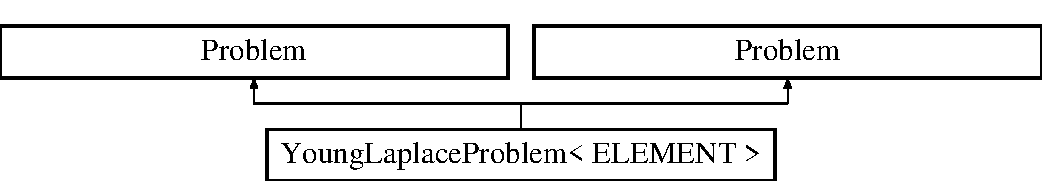
\includegraphics[height=2.000000cm]{classYoungLaplaceProblem}
\end{center}
\end{figure}
\subsection*{Public Member Functions}
\begin{DoxyCompactItemize}
\item 
\hyperlink{classYoungLaplaceProblem_a4ea552f351994849e9ab597ef2da797a}{Young\+Laplace\+Problem} ()
\begin{DoxyCompactList}\small\item\em Constructor\+: \end{DoxyCompactList}\item 
\hyperlink{classYoungLaplaceProblem_aa3482606bfd86a3db9d2dec86ba75f14}{$\sim$\+Young\+Laplace\+Problem} ()
\begin{DoxyCompactList}\small\item\em Destructor (empty) \end{DoxyCompactList}\item 
void \hyperlink{classYoungLaplaceProblem_a93dd45313d28c3b9b0b51e34d14ebd24}{actions\+\_\+before\+\_\+newton\+\_\+solve} ()
\begin{DoxyCompactList}\small\item\em Update the problem before solve. \end{DoxyCompactList}\item 
void \hyperlink{classYoungLaplaceProblem_a8eed49ad1c6247cc293a584ab9262efc}{actions\+\_\+after\+\_\+newton\+\_\+solve} ()
\begin{DoxyCompactList}\small\item\em Update the problem after solve\+: Empty. \end{DoxyCompactList}\item 
void \hyperlink{classYoungLaplaceProblem_a16f10e66457718eca76d1335dbed8f12}{doc\+\_\+solution} (Doc\+Info \&doc\+\_\+info, ofstream \&trace\+\_\+file)
\begin{DoxyCompactList}\small\item\em Doc the solution. Doc\+Info object stores flags/labels for where the output gets written to and the trace file. \end{DoxyCompactList}\item 
\hyperlink{classYoungLaplaceProblem_a4ea552f351994849e9ab597ef2da797a}{Young\+Laplace\+Problem} ()
\begin{DoxyCompactList}\small\item\em Constructor\+: \end{DoxyCompactList}\item 
\hyperlink{classYoungLaplaceProblem_aa3482606bfd86a3db9d2dec86ba75f14}{$\sim$\+Young\+Laplace\+Problem} ()
\begin{DoxyCompactList}\small\item\em Destructor (empty) \end{DoxyCompactList}\item 
void \hyperlink{classYoungLaplaceProblem_a93dd45313d28c3b9b0b51e34d14ebd24}{actions\+\_\+before\+\_\+newton\+\_\+solve} ()
\begin{DoxyCompactList}\small\item\em Update the problem specs before solve. \end{DoxyCompactList}\item 
void \hyperlink{classYoungLaplaceProblem_a8eed49ad1c6247cc293a584ab9262efc}{actions\+\_\+after\+\_\+newton\+\_\+solve} ()
\begin{DoxyCompactList}\small\item\em Update the problem after solve\+: Empty. \end{DoxyCompactList}\item 
void \hyperlink{classYoungLaplaceProblem_a16f10e66457718eca76d1335dbed8f12}{doc\+\_\+solution} (Doc\+Info \&doc\+\_\+info, ofstream \&trace\+\_\+file)
\begin{DoxyCompactList}\small\item\em Doc the solution. Doc\+Info object stores flags/labels for where the output gets written to and the trace file. \end{DoxyCompactList}\end{DoxyCompactItemize}
\subsection*{Private Member Functions}
\begin{DoxyCompactItemize}
\item 
void \hyperlink{classYoungLaplaceProblem_a3ebbc17f9f27480e720f0bd87a036a12}{create\+\_\+contact\+\_\+angle\+\_\+elements} (const unsigned \&b)
\begin{DoxyCompactList}\small\item\em Create Young\+Laplace contact angle elements on the b-\/th boundary of the problem\textquotesingle{}s mesh and add them to mesh. \end{DoxyCompactList}\end{DoxyCompactItemize}
\subsection*{Private Attributes}
\begin{DoxyCompactItemize}
\item 
Node $\ast$ \hyperlink{classYoungLaplaceProblem_a1d659f1b2d73140a5d52889f9581d12f}{Control\+\_\+node\+\_\+pt}
\begin{DoxyCompactList}\small\item\em Node at which the height (displacement along spine) is controlled/doced. \end{DoxyCompactList}\item 
Data $\ast$ \hyperlink{classYoungLaplaceProblem_a78d1ae3b73777674003b2c9794ea9b43}{Kappa\+\_\+pt}
\begin{DoxyCompactList}\small\item\em Pointer to Data object that stores the prescribed curvature. \end{DoxyCompactList}\item 
unsigned \hyperlink{classYoungLaplaceProblem_a4dc49a3807638823ac2157d67e8fed4a}{N\+\_\+bulk\+\_\+elements}
\begin{DoxyCompactList}\small\item\em Number of Young\+Laplace \char`\"{}bulk\char`\"{} elements (We\textquotesingle{}re attaching the contact angle elements to the bulk mesh --$>$ only the first N\+\_\+bulk\+\_\+elements elements in the mesh are bulk elements!) \end{DoxyCompactList}\item 
unsigned \hyperlink{classYoungLaplaceProblem_a30b767547f8b93461b56653dd007063a}{Last\+\_\+element\+\_\+on\+\_\+boundary1}
\begin{DoxyCompactList}\small\item\em Number of last Face\+Element on boundary 1. \end{DoxyCompactList}\item 
unsigned \hyperlink{classYoungLaplaceProblem_a5c9ac739e14a03c0dd36ff7407382814}{Last\+\_\+element\+\_\+on\+\_\+boundary3}
\begin{DoxyCompactList}\small\item\em Number of last Face\+Element on boundary 3. \end{DoxyCompactList}\end{DoxyCompactItemize}


\subsection{Detailed Description}
\subsubsection*{template$<$class E\+L\+E\+M\+E\+NT$>$\newline
class Young\+Laplace\+Problem$<$ E\+L\+E\+M\+E\+N\+T $>$}

2D Young\+Laplace problem on rectangular domain, discretised with 2D Q\+Young\+Laplace elements. The specific type of element is specified via the template parameter. 

Definition at line 143 of file barrel.\+cc.



\subsection{Constructor \& Destructor Documentation}
\mbox{\Hypertarget{classYoungLaplaceProblem_a4ea552f351994849e9ab597ef2da797a}\label{classYoungLaplaceProblem_a4ea552f351994849e9ab597ef2da797a}} 
\index{Young\+Laplace\+Problem@{Young\+Laplace\+Problem}!Young\+Laplace\+Problem@{Young\+Laplace\+Problem}}
\index{Young\+Laplace\+Problem@{Young\+Laplace\+Problem}!Young\+Laplace\+Problem@{Young\+Laplace\+Problem}}
\subsubsection{\texorpdfstring{Young\+Laplace\+Problem()}{YoungLaplaceProblem()}\hspace{0.1cm}{\footnotesize\ttfamily [1/2]}}
{\footnotesize\ttfamily template$<$class E\+L\+E\+M\+E\+NT $>$ \\
\hyperlink{classYoungLaplaceProblem}{Young\+Laplace\+Problem}$<$ E\+L\+E\+M\+E\+NT $>$\+::\hyperlink{classYoungLaplaceProblem}{Young\+Laplace\+Problem} (\begin{DoxyParamCaption}{ }\end{DoxyParamCaption})}



Constructor\+: 

Constructor for Young\+Laplace problem. Add height control element to mesh at the very end 

Definition at line 184 of file barrel.\+cc.



References Global\+Parameters\+::\+Controlled\+\_\+height, Global\+Parameters\+::\+Kappa\+\_\+pt, Global\+Parameters\+::spine\+\_\+base\+\_\+function(), and Global\+Parameters\+::spine\+\_\+function().

\mbox{\Hypertarget{classYoungLaplaceProblem_aa3482606bfd86a3db9d2dec86ba75f14}\label{classYoungLaplaceProblem_aa3482606bfd86a3db9d2dec86ba75f14}} 
\index{Young\+Laplace\+Problem@{Young\+Laplace\+Problem}!````~Young\+Laplace\+Problem@{$\sim$\+Young\+Laplace\+Problem}}
\index{````~Young\+Laplace\+Problem@{$\sim$\+Young\+Laplace\+Problem}!Young\+Laplace\+Problem@{Young\+Laplace\+Problem}}
\subsubsection{\texorpdfstring{$\sim$\+Young\+Laplace\+Problem()}{~YoungLaplaceProblem()}\hspace{0.1cm}{\footnotesize\ttfamily [1/2]}}
{\footnotesize\ttfamily template$<$class E\+L\+E\+M\+E\+NT$>$ \\
\hyperlink{classYoungLaplaceProblem}{Young\+Laplace\+Problem}$<$ E\+L\+E\+M\+E\+NT $>$\+::$\sim$\hyperlink{classYoungLaplaceProblem}{Young\+Laplace\+Problem} (\begin{DoxyParamCaption}{ }\end{DoxyParamCaption})\hspace{0.3cm}{\ttfamily [inline]}}



Destructor (empty) 



Definition at line 152 of file barrel.\+cc.

\mbox{\Hypertarget{classYoungLaplaceProblem_a4ea552f351994849e9ab597ef2da797a}\label{classYoungLaplaceProblem_a4ea552f351994849e9ab597ef2da797a}} 
\index{Young\+Laplace\+Problem@{Young\+Laplace\+Problem}!Young\+Laplace\+Problem@{Young\+Laplace\+Problem}}
\index{Young\+Laplace\+Problem@{Young\+Laplace\+Problem}!Young\+Laplace\+Problem@{Young\+Laplace\+Problem}}
\subsubsection{\texorpdfstring{Young\+Laplace\+Problem()}{YoungLaplaceProblem()}\hspace{0.1cm}{\footnotesize\ttfamily [2/2]}}
{\footnotesize\ttfamily template$<$class E\+L\+E\+M\+E\+NT$>$ \\
\hyperlink{classYoungLaplaceProblem}{Young\+Laplace\+Problem}$<$ E\+L\+E\+M\+E\+NT $>$\+::\hyperlink{classYoungLaplaceProblem}{Young\+Laplace\+Problem} (\begin{DoxyParamCaption}{ }\end{DoxyParamCaption})}



Constructor\+: 

\mbox{\Hypertarget{classYoungLaplaceProblem_aa3482606bfd86a3db9d2dec86ba75f14}\label{classYoungLaplaceProblem_aa3482606bfd86a3db9d2dec86ba75f14}} 
\index{Young\+Laplace\+Problem@{Young\+Laplace\+Problem}!````~Young\+Laplace\+Problem@{$\sim$\+Young\+Laplace\+Problem}}
\index{````~Young\+Laplace\+Problem@{$\sim$\+Young\+Laplace\+Problem}!Young\+Laplace\+Problem@{Young\+Laplace\+Problem}}
\subsubsection{\texorpdfstring{$\sim$\+Young\+Laplace\+Problem()}{~YoungLaplaceProblem()}\hspace{0.1cm}{\footnotesize\ttfamily [2/2]}}
{\footnotesize\ttfamily template$<$class E\+L\+E\+M\+E\+NT$>$ \\
\hyperlink{classYoungLaplaceProblem}{Young\+Laplace\+Problem}$<$ E\+L\+E\+M\+E\+NT $>$\+::$\sim$\hyperlink{classYoungLaplaceProblem}{Young\+Laplace\+Problem} (\begin{DoxyParamCaption}{ }\end{DoxyParamCaption})\hspace{0.3cm}{\ttfamily [inline]}}



Destructor (empty) 



Definition at line 66 of file young\+\_\+laplace.\+cc.



\subsection{Member Function Documentation}
\mbox{\Hypertarget{classYoungLaplaceProblem_a8eed49ad1c6247cc293a584ab9262efc}\label{classYoungLaplaceProblem_a8eed49ad1c6247cc293a584ab9262efc}} 
\index{Young\+Laplace\+Problem@{Young\+Laplace\+Problem}!actions\+\_\+after\+\_\+newton\+\_\+solve@{actions\+\_\+after\+\_\+newton\+\_\+solve}}
\index{actions\+\_\+after\+\_\+newton\+\_\+solve@{actions\+\_\+after\+\_\+newton\+\_\+solve}!Young\+Laplace\+Problem@{Young\+Laplace\+Problem}}
\subsubsection{\texorpdfstring{actions\+\_\+after\+\_\+newton\+\_\+solve()}{actions\_after\_newton\_solve()}\hspace{0.1cm}{\footnotesize\ttfamily [1/2]}}
{\footnotesize\ttfamily template$<$class E\+L\+E\+M\+E\+NT$>$ \\
void \hyperlink{classYoungLaplaceProblem}{Young\+Laplace\+Problem}$<$ E\+L\+E\+M\+E\+NT $>$\+::actions\+\_\+after\+\_\+newton\+\_\+solve (\begin{DoxyParamCaption}{ }\end{DoxyParamCaption})\hspace{0.3cm}{\ttfamily [inline]}}



Update the problem after solve\+: Empty. 



Definition at line 72 of file young\+\_\+laplace.\+cc.

\mbox{\Hypertarget{classYoungLaplaceProblem_a8eed49ad1c6247cc293a584ab9262efc}\label{classYoungLaplaceProblem_a8eed49ad1c6247cc293a584ab9262efc}} 
\index{Young\+Laplace\+Problem@{Young\+Laplace\+Problem}!actions\+\_\+after\+\_\+newton\+\_\+solve@{actions\+\_\+after\+\_\+newton\+\_\+solve}}
\index{actions\+\_\+after\+\_\+newton\+\_\+solve@{actions\+\_\+after\+\_\+newton\+\_\+solve}!Young\+Laplace\+Problem@{Young\+Laplace\+Problem}}
\subsubsection{\texorpdfstring{actions\+\_\+after\+\_\+newton\+\_\+solve()}{actions\_after\_newton\_solve()}\hspace{0.1cm}{\footnotesize\ttfamily [2/2]}}
{\footnotesize\ttfamily template$<$class E\+L\+E\+M\+E\+NT$>$ \\
void \hyperlink{classYoungLaplaceProblem}{Young\+Laplace\+Problem}$<$ E\+L\+E\+M\+E\+NT $>$\+::actions\+\_\+after\+\_\+newton\+\_\+solve (\begin{DoxyParamCaption}{ }\end{DoxyParamCaption})\hspace{0.3cm}{\ttfamily [inline]}}



Update the problem after solve\+: Empty. 



Definition at line 163 of file barrel.\+cc.

\mbox{\Hypertarget{classYoungLaplaceProblem_a93dd45313d28c3b9b0b51e34d14ebd24}\label{classYoungLaplaceProblem_a93dd45313d28c3b9b0b51e34d14ebd24}} 
\index{Young\+Laplace\+Problem@{Young\+Laplace\+Problem}!actions\+\_\+before\+\_\+newton\+\_\+solve@{actions\+\_\+before\+\_\+newton\+\_\+solve}}
\index{actions\+\_\+before\+\_\+newton\+\_\+solve@{actions\+\_\+before\+\_\+newton\+\_\+solve}!Young\+Laplace\+Problem@{Young\+Laplace\+Problem}}
\subsubsection{\texorpdfstring{actions\+\_\+before\+\_\+newton\+\_\+solve()}{actions\_before\_newton\_solve()}\hspace{0.1cm}{\footnotesize\ttfamily [1/2]}}
{\footnotesize\ttfamily template$<$class E\+L\+E\+M\+E\+NT$>$ \\
void \hyperlink{classYoungLaplaceProblem}{Young\+Laplace\+Problem}$<$ E\+L\+E\+M\+E\+NT $>$\+::actions\+\_\+before\+\_\+newton\+\_\+solve (\begin{DoxyParamCaption}{ }\end{DoxyParamCaption})}



Update the problem specs before solve. 

\mbox{\Hypertarget{classYoungLaplaceProblem_a93dd45313d28c3b9b0b51e34d14ebd24}\label{classYoungLaplaceProblem_a93dd45313d28c3b9b0b51e34d14ebd24}} 
\index{Young\+Laplace\+Problem@{Young\+Laplace\+Problem}!actions\+\_\+before\+\_\+newton\+\_\+solve@{actions\+\_\+before\+\_\+newton\+\_\+solve}}
\index{actions\+\_\+before\+\_\+newton\+\_\+solve@{actions\+\_\+before\+\_\+newton\+\_\+solve}!Young\+Laplace\+Problem@{Young\+Laplace\+Problem}}
\subsubsection{\texorpdfstring{actions\+\_\+before\+\_\+newton\+\_\+solve()}{actions\_before\_newton\_solve()}\hspace{0.1cm}{\footnotesize\ttfamily [2/2]}}
{\footnotesize\ttfamily template$<$class E\+L\+E\+M\+E\+NT $>$ \\
void \hyperlink{classYoungLaplaceProblem}{Young\+Laplace\+Problem}$<$ E\+L\+E\+M\+E\+NT $>$\+::actions\+\_\+before\+\_\+newton\+\_\+solve (\begin{DoxyParamCaption}{ }\end{DoxyParamCaption})\hspace{0.3cm}{\ttfamily [inline]}}



Update the problem before solve. 

Update the problem specs before solve\+: (Re-\/)set boundary conditions to the values from the exact solution. 

Definition at line 155 of file barrel.\+cc.



References Global\+Parameters\+::\+Kappa\+\_\+pt.



Referenced by Young\+Laplace\+Problem$<$ E\+L\+E\+M\+E\+N\+T $>$\+::create\+\_\+contact\+\_\+angle\+\_\+elements().

\mbox{\Hypertarget{classYoungLaplaceProblem_a3ebbc17f9f27480e720f0bd87a036a12}\label{classYoungLaplaceProblem_a3ebbc17f9f27480e720f0bd87a036a12}} 
\index{Young\+Laplace\+Problem@{Young\+Laplace\+Problem}!create\+\_\+contact\+\_\+angle\+\_\+elements@{create\+\_\+contact\+\_\+angle\+\_\+elements}}
\index{create\+\_\+contact\+\_\+angle\+\_\+elements@{create\+\_\+contact\+\_\+angle\+\_\+elements}!Young\+Laplace\+Problem@{Young\+Laplace\+Problem}}
\subsubsection{\texorpdfstring{create\+\_\+contact\+\_\+angle\+\_\+elements()}{create\_contact\_angle\_elements()}}
{\footnotesize\ttfamily template$<$class E\+L\+E\+M\+E\+NT $>$ \\
void \hyperlink{classYoungLaplaceProblem}{Young\+Laplace\+Problem}$<$ E\+L\+E\+M\+E\+NT $>$\+::create\+\_\+contact\+\_\+angle\+\_\+elements (\begin{DoxyParamCaption}\item[{const unsigned \&}]{b }\end{DoxyParamCaption})\hspace{0.3cm}{\ttfamily [private]}}



Create Young\+Laplace contact angle elements on the b-\/th boundary of the problem\textquotesingle{}s mesh and add them to mesh. 

Create Young\+Laplace contact angle elements on the b-\/th boundary of the Mesh. 

Definition at line 283 of file young\+\_\+laplace.\+cc.



References Young\+Laplace\+Problem$<$ E\+L\+E\+M\+E\+N\+T $>$\+::actions\+\_\+before\+\_\+newton\+\_\+solve(), Global\+Parameters\+::\+Case, Global\+Parameters\+::\+Controlled\+\_\+height, Global\+Parameters\+::\+Controlled\+\_\+height\+\_\+increment, Young\+Laplace\+Problem$<$ E\+L\+E\+M\+E\+N\+T $>$\+::doc\+\_\+solution(), Global\+Parameters\+::get\+\_\+exact\+\_\+kappa(), Global\+Parameters\+::\+Kappa\+\_\+increment, Global\+Parameters\+::\+Kappa\+\_\+pt, Global\+Parameters\+::\+T\+\_\+junction\+\_\+with\+\_\+nonzero\+\_\+contact\+\_\+angle, and Global\+Parameters\+::\+Use\+\_\+height\+\_\+control.

\mbox{\Hypertarget{classYoungLaplaceProblem_a16f10e66457718eca76d1335dbed8f12}\label{classYoungLaplaceProblem_a16f10e66457718eca76d1335dbed8f12}} 
\index{Young\+Laplace\+Problem@{Young\+Laplace\+Problem}!doc\+\_\+solution@{doc\+\_\+solution}}
\index{doc\+\_\+solution@{doc\+\_\+solution}!Young\+Laplace\+Problem@{Young\+Laplace\+Problem}}
\subsubsection{\texorpdfstring{doc\+\_\+solution()}{doc\_solution()}\hspace{0.1cm}{\footnotesize\ttfamily [1/2]}}
{\footnotesize\ttfamily template$<$class E\+L\+E\+M\+E\+NT$>$ \\
void \hyperlink{classYoungLaplaceProblem}{Young\+Laplace\+Problem}$<$ E\+L\+E\+M\+E\+NT $>$\+::doc\+\_\+solution (\begin{DoxyParamCaption}\item[{Doc\+Info \&}]{doc\+\_\+info,  }\item[{ofstream \&}]{trace\+\_\+file }\end{DoxyParamCaption})}



Doc the solution. Doc\+Info object stores flags/labels for where the output gets written to and the trace file. 

\mbox{\Hypertarget{classYoungLaplaceProblem_a16f10e66457718eca76d1335dbed8f12}\label{classYoungLaplaceProblem_a16f10e66457718eca76d1335dbed8f12}} 
\index{Young\+Laplace\+Problem@{Young\+Laplace\+Problem}!doc\+\_\+solution@{doc\+\_\+solution}}
\index{doc\+\_\+solution@{doc\+\_\+solution}!Young\+Laplace\+Problem@{Young\+Laplace\+Problem}}
\subsubsection{\texorpdfstring{doc\+\_\+solution()}{doc\_solution()}\hspace{0.1cm}{\footnotesize\ttfamily [2/2]}}
{\footnotesize\ttfamily template$<$class E\+L\+E\+M\+E\+NT $>$ \\
void \hyperlink{classYoungLaplaceProblem}{Young\+Laplace\+Problem}$<$ E\+L\+E\+M\+E\+NT $>$\+::doc\+\_\+solution (\begin{DoxyParamCaption}\item[{Doc\+Info \&}]{doc\+\_\+info,  }\item[{ofstream \&}]{trace\+\_\+file }\end{DoxyParamCaption})}



Doc the solution. Doc\+Info object stores flags/labels for where the output gets written to and the trace file. 

Doc the solution\+: doc\+\_\+info contains labels/output directory etc. 

Definition at line 295 of file barrel.\+cc.



References Global\+Parameters\+::get\+\_\+exact\+\_\+kappa(), and Global\+Parameters\+::\+Kappa\+\_\+pt.



Referenced by Young\+Laplace\+Problem$<$ E\+L\+E\+M\+E\+N\+T $>$\+::create\+\_\+contact\+\_\+angle\+\_\+elements(), main(), and run\+\_\+it().



\subsection{Member Data Documentation}
\mbox{\Hypertarget{classYoungLaplaceProblem_a1d659f1b2d73140a5d52889f9581d12f}\label{classYoungLaplaceProblem_a1d659f1b2d73140a5d52889f9581d12f}} 
\index{Young\+Laplace\+Problem@{Young\+Laplace\+Problem}!Control\+\_\+node\+\_\+pt@{Control\+\_\+node\+\_\+pt}}
\index{Control\+\_\+node\+\_\+pt@{Control\+\_\+node\+\_\+pt}!Young\+Laplace\+Problem@{Young\+Laplace\+Problem}}
\subsubsection{\texorpdfstring{Control\+\_\+node\+\_\+pt}{Control\_node\_pt}}
{\footnotesize\ttfamily template$<$class E\+L\+E\+M\+E\+NT$>$ \\
Node $\ast$ \hyperlink{classYoungLaplaceProblem}{Young\+Laplace\+Problem}$<$ E\+L\+E\+M\+E\+NT $>$\+::Control\+\_\+node\+\_\+pt\hspace{0.3cm}{\ttfamily [private]}}



Node at which the height (displacement along spine) is controlled/doced. 



Definition at line 172 of file barrel.\+cc.

\mbox{\Hypertarget{classYoungLaplaceProblem_a78d1ae3b73777674003b2c9794ea9b43}\label{classYoungLaplaceProblem_a78d1ae3b73777674003b2c9794ea9b43}} 
\index{Young\+Laplace\+Problem@{Young\+Laplace\+Problem}!Kappa\+\_\+pt@{Kappa\+\_\+pt}}
\index{Kappa\+\_\+pt@{Kappa\+\_\+pt}!Young\+Laplace\+Problem@{Young\+Laplace\+Problem}}
\subsubsection{\texorpdfstring{Kappa\+\_\+pt}{Kappa\_pt}}
{\footnotesize\ttfamily template$<$class E\+L\+E\+M\+E\+NT$>$ \\
Data$\ast$ \hyperlink{classYoungLaplaceProblem}{Young\+Laplace\+Problem}$<$ E\+L\+E\+M\+E\+NT $>$\+::Kappa\+\_\+pt\hspace{0.3cm}{\ttfamily [private]}}



Pointer to Data object that stores the prescribed curvature. 



Definition at line 175 of file barrel.\+cc.

\mbox{\Hypertarget{classYoungLaplaceProblem_a30b767547f8b93461b56653dd007063a}\label{classYoungLaplaceProblem_a30b767547f8b93461b56653dd007063a}} 
\index{Young\+Laplace\+Problem@{Young\+Laplace\+Problem}!Last\+\_\+element\+\_\+on\+\_\+boundary1@{Last\+\_\+element\+\_\+on\+\_\+boundary1}}
\index{Last\+\_\+element\+\_\+on\+\_\+boundary1@{Last\+\_\+element\+\_\+on\+\_\+boundary1}!Young\+Laplace\+Problem@{Young\+Laplace\+Problem}}
\subsubsection{\texorpdfstring{Last\+\_\+element\+\_\+on\+\_\+boundary1}{Last\_element\_on\_boundary1}}
{\footnotesize\ttfamily template$<$class E\+L\+E\+M\+E\+NT$>$ \\
unsigned \hyperlink{classYoungLaplaceProblem}{Young\+Laplace\+Problem}$<$ E\+L\+E\+M\+E\+NT $>$\+::Last\+\_\+element\+\_\+on\+\_\+boundary1\hspace{0.3cm}{\ttfamily [private]}}



Number of last Face\+Element on boundary 1. 



Definition at line 90 of file young\+\_\+laplace.\+cc.

\mbox{\Hypertarget{classYoungLaplaceProblem_a5c9ac739e14a03c0dd36ff7407382814}\label{classYoungLaplaceProblem_a5c9ac739e14a03c0dd36ff7407382814}} 
\index{Young\+Laplace\+Problem@{Young\+Laplace\+Problem}!Last\+\_\+element\+\_\+on\+\_\+boundary3@{Last\+\_\+element\+\_\+on\+\_\+boundary3}}
\index{Last\+\_\+element\+\_\+on\+\_\+boundary3@{Last\+\_\+element\+\_\+on\+\_\+boundary3}!Young\+Laplace\+Problem@{Young\+Laplace\+Problem}}
\subsubsection{\texorpdfstring{Last\+\_\+element\+\_\+on\+\_\+boundary3}{Last\_element\_on\_boundary3}}
{\footnotesize\ttfamily template$<$class E\+L\+E\+M\+E\+NT$>$ \\
unsigned \hyperlink{classYoungLaplaceProblem}{Young\+Laplace\+Problem}$<$ E\+L\+E\+M\+E\+NT $>$\+::Last\+\_\+element\+\_\+on\+\_\+boundary3\hspace{0.3cm}{\ttfamily [private]}}



Number of last Face\+Element on boundary 3. 



Definition at line 93 of file young\+\_\+laplace.\+cc.

\mbox{\Hypertarget{classYoungLaplaceProblem_a4dc49a3807638823ac2157d67e8fed4a}\label{classYoungLaplaceProblem_a4dc49a3807638823ac2157d67e8fed4a}} 
\index{Young\+Laplace\+Problem@{Young\+Laplace\+Problem}!N\+\_\+bulk\+\_\+elements@{N\+\_\+bulk\+\_\+elements}}
\index{N\+\_\+bulk\+\_\+elements@{N\+\_\+bulk\+\_\+elements}!Young\+Laplace\+Problem@{Young\+Laplace\+Problem}}
\subsubsection{\texorpdfstring{N\+\_\+bulk\+\_\+elements}{N\_bulk\_elements}}
{\footnotesize\ttfamily template$<$class E\+L\+E\+M\+E\+NT$>$ \\
unsigned \hyperlink{classYoungLaplaceProblem}{Young\+Laplace\+Problem}$<$ E\+L\+E\+M\+E\+NT $>$\+::N\+\_\+bulk\+\_\+elements\hspace{0.3cm}{\ttfamily [private]}}



Number of Young\+Laplace \char`\"{}bulk\char`\"{} elements (We\textquotesingle{}re attaching the contact angle elements to the bulk mesh --$>$ only the first N\+\_\+bulk\+\_\+elements elements in the mesh are bulk elements!) 



Definition at line 87 of file young\+\_\+laplace.\+cc.



The documentation for this class was generated from the following files\+:\begin{DoxyCompactItemize}
\item 
\hyperlink{barrel_8cc}{barrel.\+cc}\item 
\hyperlink{young__laplace_8cc}{young\+\_\+laplace.\+cc}\end{DoxyCompactItemize}

\chapter{File Documentation}
\hypertarget{barrel_8cc}{}\section{barrel.\+cc File Reference}
\label{barrel_8cc}\index{barrel.\+cc@{barrel.\+cc}}
\subsection*{Classes}
\begin{DoxyCompactItemize}
\item 
class \hyperlink{classYoungLaplaceProblem}{Young\+Laplace\+Problem$<$ E\+L\+E\+M\+E\+N\+T $>$}
\end{DoxyCompactItemize}
\subsection*{Namespaces}
\begin{DoxyCompactItemize}
\item 
 \hyperlink{namespaceGlobalParameters}{Global\+Parameters}
\begin{DoxyCompactList}\small\item\em Namespace for \char`\"{}global\char`\"{} problem parameters. \end{DoxyCompactList}\end{DoxyCompactItemize}
\subsection*{Functions}
\begin{DoxyCompactItemize}
\item 
double \hyperlink{namespaceGlobalParameters_a4571d41514b16946dd31d075d44c5593}{Global\+Parameters\+::get\+\_\+exact\+\_\+kappa} ()
\begin{DoxyCompactList}\small\item\em Exact kappa. \end{DoxyCompactList}\item 
void \hyperlink{namespaceGlobalParameters_ac81daf87f8d3f075d9fd108427e70c4f}{Global\+Parameters\+::spine\+\_\+base\+\_\+function} (const Vector$<$ double $>$ \&x, Vector$<$ double $>$ \&spine\+\_\+B, Vector$<$ Vector$<$ double $>$ $>$ \&dspine\+\_\+B)
\begin{DoxyCompactList}\small\item\em Spine basis\+: The position vector to the basis of the spine as a function of the two coordinates x\+\_\+1 and x\+\_\+2, and its derivatives w.\+r.\+t. to these coordinates. dspine\+\_\+B\mbox{[}i\mbox{]}\mbox{[}j\mbox{]} = d spine\+\_\+B\mbox{[}j\mbox{]} / dx\+\_\+i Spines start in the (x\+\_\+1,x\+\_\+2) plane at (x\+\_\+1,x\+\_\+2). \end{DoxyCompactList}\item 
void \hyperlink{namespaceGlobalParameters_a82df8c67f58e78a236fb6a0cc8bf8284}{Global\+Parameters\+::spine\+\_\+function} (const Vector$<$ double $>$ \&x, Vector$<$ double $>$ \&spine, Vector$<$ Vector$<$ double $>$ $>$ \&dspine)
\begin{DoxyCompactList}\small\item\em Spine\+: The spine vector field as a function of the two coordinates x\+\_\+1 and x\+\_\+2, and its derivatives w.\+r.\+t. to these coordinates\+: dspine\mbox{[}i\mbox{]}\mbox{[}j\mbox{]} = d spine\mbox{[}j\mbox{]} / dx\+\_\+i. \end{DoxyCompactList}\item 
int \hyperlink{barrel_8cc_ae66f6b31b5ad750f1fe042a706a4e3d4}{main} ()
\begin{DoxyCompactList}\small\item\em Driver code. \end{DoxyCompactList}\end{DoxyCompactItemize}
\subsection*{Variables}
\begin{DoxyCompactItemize}
\item 
double \hyperlink{namespaceGlobalParameters_a3731f24a02ce4f306d65a9a488f85c96}{Global\+Parameters\+::\+Controlled\+\_\+height} = 0.\+0
\begin{DoxyCompactList}\small\item\em Height control value. \end{DoxyCompactList}\item 
double \hyperlink{namespaceGlobalParameters_ae8fa7610a34b7a2a8223eade99a5c22f}{Global\+Parameters\+::\+Alpha\+\_\+min} = Mathematical\+Constants\+::\+Pi/2.\+0$\ast$1.\+5
\begin{DoxyCompactList}\small\item\em Min. spine angle against horizontal plane. \end{DoxyCompactList}\item 
double \hyperlink{namespaceGlobalParameters_a19d04a02b0b5ef5c72e9c30d822e4dc7}{Global\+Parameters\+::\+Alpha\+\_\+max} = Mathematical\+Constants\+::\+Pi/2.\+0$\ast$0.\+5
\begin{DoxyCompactList}\small\item\em Max. spine angle against horizontal plane. \end{DoxyCompactList}\end{DoxyCompactItemize}


\subsection{Function Documentation}
\mbox{\Hypertarget{barrel_8cc_ae66f6b31b5ad750f1fe042a706a4e3d4}\label{barrel_8cc_ae66f6b31b5ad750f1fe042a706a4e3d4}} 
\index{barrel.\+cc@{barrel.\+cc}!main@{main}}
\index{main@{main}!barrel.\+cc@{barrel.\+cc}}
\subsubsection{\texorpdfstring{main()}{main()}}
{\footnotesize\ttfamily int main (\begin{DoxyParamCaption}{ }\end{DoxyParamCaption})}



Driver code. 



Definition at line 325 of file barrel.\+cc.



References Global\+Parameters\+::\+Controlled\+\_\+height, and Young\+Laplace\+Problem$<$ E\+L\+E\+M\+E\+N\+T $>$\+::doc\+\_\+solution().


\hypertarget{common__young__laplace__stuff_8h}{}\section{common\+\_\+young\+\_\+laplace\+\_\+stuff.\+h File Reference}
\label{common__young__laplace__stuff_8h}\index{common\+\_\+young\+\_\+laplace\+\_\+stuff.\+h@{common\+\_\+young\+\_\+laplace\+\_\+stuff.\+h}}
\subsection*{Namespaces}
\begin{DoxyCompactItemize}
\item 
 \hyperlink{namespaceGlobalParameters}{Global\+Parameters}
\begin{DoxyCompactList}\small\item\em Namespace for \char`\"{}global\char`\"{} problem parameters. \end{DoxyCompactList}\end{DoxyCompactItemize}
\subsection*{Enumerations}
\begin{DoxyCompactItemize}
\item 
enum \hyperlink{namespaceGlobalParameters_adde04e4243b82e3d4bd2f82d37a2d6bf}{Global\+Parameters\+::\+Cases} \{ \hyperlink{namespaceGlobalParameters_adde04e4243b82e3d4bd2f82d37a2d6bfac08080f634c714da38f1122301eafda7}{Global\+Parameters\+::\+Spherical\+\_\+cap\+\_\+in\+\_\+cylinder\+\_\+pinned}, 
\hyperlink{namespaceGlobalParameters_adde04e4243b82e3d4bd2f82d37a2d6bfa28147edc9cfc06038f2a7deaf8890558}{Global\+Parameters\+::\+All\+\_\+pinned}, 
\hyperlink{namespaceGlobalParameters_adde04e4243b82e3d4bd2f82d37a2d6bfa1e6d2261f2fa0541d57b5a0a8c044ddc}{Global\+Parameters\+::\+Barrel\+\_\+shape}, 
\hyperlink{namespaceGlobalParameters_adde04e4243b82e3d4bd2f82d37a2d6bfa89cfbba408c0774e0b9024baa187dfb8}{Global\+Parameters\+::\+T\+\_\+junction\+\_\+with\+\_\+nonzero\+\_\+contact\+\_\+angle}
 \}\begin{DoxyCompactList}\small\item\em Enumeration for the possible cases. \end{DoxyCompactList}
\end{DoxyCompactItemize}
\subsection*{Functions}
\begin{DoxyCompactItemize}
\item 
void \hyperlink{namespaceGlobalParameters_aedbc21f2c81d445634badfc5cdd77436}{Global\+Parameters\+::setup\+\_\+dependent\+\_\+parameters\+\_\+and\+\_\+sanity\+\_\+check} ()
\begin{DoxyCompactList}\small\item\em Setup dependent parameters and perform sanity check. \end{DoxyCompactList}\item 
void \hyperlink{namespaceGlobalParameters_ac81daf87f8d3f075d9fd108427e70c4f}{Global\+Parameters\+::spine\+\_\+base\+\_\+function} (const Vector$<$ double $>$ \&x, Vector$<$ double $>$ \&spine\+\_\+B, Vector$<$ Vector$<$ double $>$ $>$ \&dspine\+\_\+B)
\begin{DoxyCompactList}\small\item\em Spine basis\+: The position vector to the basis of the spine as a function of the two coordinates x\+\_\+1 and x\+\_\+2, and its derivatives w.\+r.\+t. to these coordinates. dspine\+\_\+B\mbox{[}i\mbox{]}\mbox{[}j\mbox{]} = d spine\+\_\+B\mbox{[}j\mbox{]} / dx\+\_\+i Spines start in the (x\+\_\+1,x\+\_\+2) plane at (x\+\_\+1,x\+\_\+2). \end{DoxyCompactList}\item 
void \hyperlink{namespaceGlobalParameters_a82df8c67f58e78a236fb6a0cc8bf8284}{Global\+Parameters\+::spine\+\_\+function} (const Vector$<$ double $>$ \&x, Vector$<$ double $>$ \&spine, Vector$<$ Vector$<$ double $>$ $>$ \&dspine)
\begin{DoxyCompactList}\small\item\em Spine\+: The spine vector field as a function of the two coordinates x\+\_\+1 and x\+\_\+2, and its derivatives w.\+r.\+t. to these coordinates\+: dspine\mbox{[}i\mbox{]}\mbox{[}j\mbox{]} = d spine\mbox{[}j\mbox{]} / dx\+\_\+i. \end{DoxyCompactList}\item 
double \hyperlink{namespaceGlobalParameters_a4571d41514b16946dd31d075d44c5593}{Global\+Parameters\+::get\+\_\+exact\+\_\+kappa} ()
\begin{DoxyCompactList}\small\item\em Exact kappa. \end{DoxyCompactList}\end{DoxyCompactItemize}
\subsection*{Variables}
\begin{DoxyCompactItemize}
\item 
bool \hyperlink{namespaceGlobalParameters_a7cd7766fae9d0ca421d7e24677be3131}{Global\+Parameters\+::\+Use\+\_\+spines} = true
\begin{DoxyCompactList}\small\item\em Use spines (true) or not (false) \end{DoxyCompactList}\item 
bool \hyperlink{namespaceGlobalParameters_a624713d35bc418b2d5fa79f4d385a27a}{Global\+Parameters\+::\+Use\+\_\+height\+\_\+control} = true
\begin{DoxyCompactList}\small\item\em Use height control (true) or not (false)? \end{DoxyCompactList}\item 
int \hyperlink{namespaceGlobalParameters_aeb4257eec7a4c5a92e2b88e93248a201}{Global\+Parameters\+::\+Case} = All\+\_\+pinned
\begin{DoxyCompactList}\small\item\em What case are we considering\+: Choose one from the enumeration Cases. \end{DoxyCompactList}\item 
double \hyperlink{namespaceGlobalParameters_adb0a994119055242fcc762cac5edc317}{Global\+Parameters\+::\+Gamma} = Mathematical\+Constants\+::\+Pi/4.\+0
\begin{DoxyCompactList}\small\item\em Contact angle and its cos (dependent parameter -- is reassigned) \end{DoxyCompactList}\item 
double \hyperlink{namespaceGlobalParameters_ae982fcb894e82c683d07d3c2fbbead3d}{Global\+Parameters\+::\+Cos\+\_\+gamma} =cos(Gamma)
\begin{DoxyCompactList}\small\item\em Cos of contact angle. \end{DoxyCompactList}\item 
Data $\ast$ \hyperlink{namespaceGlobalParameters_ac6234184cce40ab2c6bec92b37e4ae41}{Global\+Parameters\+::\+Kappa\+\_\+pt} = 0
\begin{DoxyCompactList}\small\item\em Pointer to Data object that stores the prescribed curvature. \end{DoxyCompactList}\item 
double \hyperlink{namespaceGlobalParameters_ae7651e73d3f8346da9fcfdbb149bc22e}{Global\+Parameters\+::\+Kappa\+\_\+initial} = 0.\+0
\begin{DoxyCompactList}\small\item\em Initial value for kappa. \end{DoxyCompactList}\item 
int \hyperlink{namespaceGlobalParameters_aeb81cc1c282502497ef6df576559b650}{Global\+Parameters\+::\+Step\+\_\+sign} = 1
\begin{DoxyCompactList}\small\item\em Increase or decrease the value of the control parameters? \end{DoxyCompactList}\item 
unsigned \hyperlink{namespaceGlobalParameters_aa6c94936d7c81286bb747e14a90d7ba0}{Global\+Parameters\+::\+Nsteps} = 5
\begin{DoxyCompactList}\small\item\em Number of steps. \end{DoxyCompactList}\item 
double \hyperlink{namespaceGlobalParameters_a74cc88d6dc206cd556fb12e7e3101032}{Global\+Parameters\+::\+Kappa\+\_\+increment} = -\/0.\+05
\begin{DoxyCompactList}\small\item\em Increment for prescribed curvature. \end{DoxyCompactList}\item 
double \hyperlink{namespaceGlobalParameters_a65fe7fd6c6c54d7ba89fab47cd4a9141}{Global\+Parameters\+::\+Controlled\+\_\+height\+\_\+increment} = 0.\+1
\begin{DoxyCompactList}\small\item\em Increment for height control. \end{DoxyCompactList}\item 
unsigned \hyperlink{namespaceGlobalParameters_a3a90a762edbce6d2a95456df26e85cea}{Global\+Parameters\+::\+Control\+\_\+element} = 0
\item 
double \hyperlink{namespaceGlobalParameters_a36ebf514fdd1e78fff69907b39e25af6}{Global\+Parameters\+::\+L\+\_\+x} = 1.\+0
\begin{DoxyCompactList}\small\item\em Length and width of the domain. \end{DoxyCompactList}\item 
double \hyperlink{namespaceGlobalParameters_ac8774b3418c4551091d64ec72c169b2e}{Global\+Parameters\+::\+L\+\_\+y} = 1.\+0
\begin{DoxyCompactList}\small\item\em Width of domain. \end{DoxyCompactList}\item 
unsigned \hyperlink{namespaceGlobalParameters_ab020cb50fa321b26e8d2127d2cff23b9}{Global\+Parameters\+::\+N\+\_\+x} = 8
\begin{DoxyCompactList}\small\item\em Number of elements in the mesh. \end{DoxyCompactList}\item 
unsigned \hyperlink{namespaceGlobalParameters_a711d6f05552ddaac30bd245ae8bdf878}{Global\+Parameters\+::\+N\+\_\+y} = 8
\item 
double \hyperlink{namespaceGlobalParameters_aeb7f1ae574be563e0b603662c6fff5aa}{Global\+Parameters\+::\+Beta\+\_\+min} = Mathematical\+Constants\+::\+Pi/2.\+0
\begin{DoxyCompactList}\small\item\em Min. second spine angle against horizontal plane. \end{DoxyCompactList}\item 
double \hyperlink{namespaceGlobalParameters_aa34aff6eb29a2a1245e9ffc2fac42caa}{Global\+Parameters\+::\+Beta\+\_\+max} = Mathematical\+Constants\+::\+Pi/2.\+0
\begin{DoxyCompactList}\small\item\em Max. second pine angle against horizontal plane. \end{DoxyCompactList}\item 
bool \hyperlink{namespaceGlobalParameters_a69a238365a4fef33b1abdae287185f3e}{Global\+Parameters\+::\+Rotate\+\_\+spines\+\_\+in\+\_\+both\+\_\+directions} = true
\begin{DoxyCompactList}\small\item\em Should the spines rotate in the x and y directions (true)? \end{DoxyCompactList}\end{DoxyCompactItemize}

\hypertarget{contact__angle_8txt__doxygenified_8h}{}\section{contact\+\_\+angle.\+txt\+\_\+doxygenified.\+h File Reference}
\label{contact__angle_8txt__doxygenified_8h}\index{contact\+\_\+angle.\+txt\+\_\+doxygenified.\+h@{contact\+\_\+angle.\+txt\+\_\+doxygenified.\+h}}

\hypertarget{refineable__t__junction_8cc}{}\section{refineable\+\_\+t\+\_\+junction.\+cc File Reference}
\label{refineable__t__junction_8cc}\index{refineable\+\_\+t\+\_\+junction.\+cc@{refineable\+\_\+t\+\_\+junction.\+cc}}
\subsection*{Classes}
\begin{DoxyCompactItemize}
\item 
class \hyperlink{classRefineableYoungLaplaceProblem}{Refineable\+Young\+Laplace\+Problem$<$ E\+L\+E\+M\+E\+N\+T $>$}
\end{DoxyCompactItemize}
\subsection*{Namespaces}
\begin{DoxyCompactItemize}
\item 
 \hyperlink{namespaceGlobalParameters}{Global\+Parameters}
\begin{DoxyCompactList}\small\item\em Namespace for \char`\"{}global\char`\"{} problem parameters. \end{DoxyCompactList}\end{DoxyCompactItemize}
\subsection*{Functions}
\begin{DoxyCompactItemize}
\item 
void \hyperlink{namespaceGlobalParameters_ac81daf87f8d3f075d9fd108427e70c4f}{Global\+Parameters\+::spine\+\_\+base\+\_\+function} (const Vector$<$ double $>$ \&x, Vector$<$ double $>$ \&spine\+\_\+B, Vector$<$ Vector$<$ double $>$ $>$ \&dspine\+\_\+B)
\begin{DoxyCompactList}\small\item\em Spine basis\+: The position vector to the basis of the spine as a function of the two coordinates x\+\_\+1 and x\+\_\+2, and its derivatives w.\+r.\+t. to these coordinates. dspine\+\_\+B\mbox{[}i\mbox{]}\mbox{[}j\mbox{]} = d spine\+\_\+B\mbox{[}j\mbox{]} / dx\+\_\+i Spines start in the (x\+\_\+1,x\+\_\+2) plane at (x\+\_\+1,x\+\_\+2). \end{DoxyCompactList}\item 
void \hyperlink{namespaceGlobalParameters_a82df8c67f58e78a236fb6a0cc8bf8284}{Global\+Parameters\+::spine\+\_\+function} (const Vector$<$ double $>$ \&x, Vector$<$ double $>$ \&spine, Vector$<$ Vector$<$ double $>$ $>$ \&dspine)
\begin{DoxyCompactList}\small\item\em Spine\+: The spine vector field as a function of the two coordinates x\+\_\+1 and x\+\_\+2, and its derivatives w.\+r.\+t. to these coordinates\+: dspine\mbox{[}i\mbox{]}\mbox{[}j\mbox{]} = d spine\mbox{[}j\mbox{]} / dx\+\_\+i. \end{DoxyCompactList}\item 
int \hyperlink{refineable__t__junction_8cc_ae66f6b31b5ad750f1fe042a706a4e3d4}{main} ()
\begin{DoxyCompactList}\small\item\em Drive code. \end{DoxyCompactList}\end{DoxyCompactItemize}


\subsection{Function Documentation}
\mbox{\Hypertarget{refineable__t__junction_8cc_ae66f6b31b5ad750f1fe042a706a4e3d4}\label{refineable__t__junction_8cc_ae66f6b31b5ad750f1fe042a706a4e3d4}} 
\index{refineable\+\_\+t\+\_\+junction.\+cc@{refineable\+\_\+t\+\_\+junction.\+cc}!main@{main}}
\index{main@{main}!refineable\+\_\+t\+\_\+junction.\+cc@{refineable\+\_\+t\+\_\+junction.\+cc}}
\subsubsection{\texorpdfstring{main()}{main()}}
{\footnotesize\ttfamily int main (\begin{DoxyParamCaption}{ }\end{DoxyParamCaption})}



Drive code. 



Definition at line 547 of file refineable\+\_\+t\+\_\+junction.\+cc.



References Global\+Parameters\+::\+Controlled\+\_\+height, and Refineable\+Young\+Laplace\+Problem$<$ E\+L\+E\+M\+E\+N\+T $>$\+::doc\+\_\+solution().


\hypertarget{refineable__young__laplace_8cc}{}\section{refineable\+\_\+young\+\_\+laplace.\+cc File Reference}
\label{refineable__young__laplace_8cc}\index{refineable\+\_\+young\+\_\+laplace.\+cc@{refineable\+\_\+young\+\_\+laplace.\+cc}}
\subsection*{Classes}
\begin{DoxyCompactItemize}
\item 
class \hyperlink{classRefineableYoungLaplaceProblem}{Refineable\+Young\+Laplace\+Problem$<$ E\+L\+E\+M\+E\+N\+T $>$}
\end{DoxyCompactItemize}
\subsection*{Functions}
\begin{DoxyCompactItemize}
\item 
void \hyperlink{refineable__young__laplace_8cc_ae164cec5b3a54dd85b4b4f36ad5cb1e2}{run\+\_\+it} (const string \&output\+\_\+directory)
\item 
int \hyperlink{refineable__young__laplace_8cc_a0ddf1224851353fc92bfbff6f499fa97}{main} (int argc, char $\ast$argv\mbox{[}$\,$\mbox{]})
\end{DoxyCompactItemize}


\subsection{Function Documentation}
\mbox{\Hypertarget{refineable__young__laplace_8cc_a0ddf1224851353fc92bfbff6f499fa97}\label{refineable__young__laplace_8cc_a0ddf1224851353fc92bfbff6f499fa97}} 
\index{refineable\+\_\+young\+\_\+laplace.\+cc@{refineable\+\_\+young\+\_\+laplace.\+cc}!main@{main}}
\index{main@{main}!refineable\+\_\+young\+\_\+laplace.\+cc@{refineable\+\_\+young\+\_\+laplace.\+cc}}
\subsubsection{\texorpdfstring{main()}{main()}}
{\footnotesize\ttfamily int main (\begin{DoxyParamCaption}\item[{int}]{argc,  }\item[{char $\ast$}]{argv\mbox{[}$\,$\mbox{]} }\end{DoxyParamCaption})}

Driver code for 2D Refineable\+Young\+Laplace problem. Input arguments\+: none (for validation) or case (0,1,2,3 for all pinned, barrel with spines, barrel without spines, and T junction), and number of steps. 

Definition at line 620 of file refineable\+\_\+young\+\_\+laplace.\+cc.



References Global\+Parameters\+::\+All\+\_\+pinned, Global\+Parameters\+::\+Barrel\+\_\+shape, Global\+Parameters\+::\+Case, Global\+Parameters\+::\+Controlled\+\_\+height\+\_\+increment, Global\+Parameters\+::\+Gamma, Global\+Parameters\+::\+L\+\_\+x, Global\+Parameters\+::\+L\+\_\+y, Global\+Parameters\+::\+Nsteps, run\+\_\+it(), Global\+Parameters\+::\+T\+\_\+junction\+\_\+with\+\_\+nonzero\+\_\+contact\+\_\+angle, and Global\+Parameters\+::\+Use\+\_\+spines.

\mbox{\Hypertarget{refineable__young__laplace_8cc_ae164cec5b3a54dd85b4b4f36ad5cb1e2}\label{refineable__young__laplace_8cc_ae164cec5b3a54dd85b4b4f36ad5cb1e2}} 
\index{refineable\+\_\+young\+\_\+laplace.\+cc@{refineable\+\_\+young\+\_\+laplace.\+cc}!run\+\_\+it@{run\+\_\+it}}
\index{run\+\_\+it@{run\+\_\+it}!refineable\+\_\+young\+\_\+laplace.\+cc@{refineable\+\_\+young\+\_\+laplace.\+cc}}
\subsubsection{\texorpdfstring{run\+\_\+it()}{run\_it()}}
{\footnotesize\ttfamily void run\+\_\+it (\begin{DoxyParamCaption}\item[{const string \&}]{output\+\_\+directory }\end{DoxyParamCaption})}

Run code for current setting of parameter values -- specify name of output directory 

Definition at line 545 of file refineable\+\_\+young\+\_\+laplace.\+cc.



References Refineable\+Young\+Laplace\+Problem$<$ E\+L\+E\+M\+E\+N\+T $>$\+::doc\+\_\+solution(), Refineable\+Young\+Laplace\+Problem$<$ E\+L\+E\+M\+E\+N\+T $>$\+::increment\+\_\+parameters(), and Global\+Parameters\+::\+Nsteps.



Referenced by main().


\hypertarget{spherical__cap__in__cylinder_8cc}{}\section{spherical\+\_\+cap\+\_\+in\+\_\+cylinder.\+cc File Reference}
\label{spherical__cap__in__cylinder_8cc}\index{spherical\+\_\+cap\+\_\+in\+\_\+cylinder.\+cc@{spherical\+\_\+cap\+\_\+in\+\_\+cylinder.\+cc}}
\subsection*{Classes}
\begin{DoxyCompactItemize}
\item 
class \hyperlink{classRefineableYoungLaplaceProblem}{Refineable\+Young\+Laplace\+Problem$<$ E\+L\+E\+M\+E\+N\+T $>$}
\end{DoxyCompactItemize}
\subsection*{Functions}
\begin{DoxyCompactItemize}
\item 
int \hyperlink{spherical__cap__in__cylinder_8cc_a0ddf1224851353fc92bfbff6f499fa97}{main} (int argc, char $\ast$argv\mbox{[}$\,$\mbox{]})
\end{DoxyCompactItemize}


\subsection{Function Documentation}
\mbox{\Hypertarget{spherical__cap__in__cylinder_8cc_a0ddf1224851353fc92bfbff6f499fa97}\label{spherical__cap__in__cylinder_8cc_a0ddf1224851353fc92bfbff6f499fa97}} 
\index{spherical\+\_\+cap\+\_\+in\+\_\+cylinder.\+cc@{spherical\+\_\+cap\+\_\+in\+\_\+cylinder.\+cc}!main@{main}}
\index{main@{main}!spherical\+\_\+cap\+\_\+in\+\_\+cylinder.\+cc@{spherical\+\_\+cap\+\_\+in\+\_\+cylinder.\+cc}}
\subsubsection{\texorpdfstring{main()}{main()}}
{\footnotesize\ttfamily int main (\begin{DoxyParamCaption}\item[{int}]{argc,  }\item[{char $\ast$}]{argv\mbox{[}$\,$\mbox{]} }\end{DoxyParamCaption})}

Driver code for 2D Refineable\+Young\+Laplace problem. Input arguments\+: none (for validation) or number of steps. 

Definition at line 292 of file spherical\+\_\+cap\+\_\+in\+\_\+cylinder.\+cc.



References Global\+Parameters\+::\+Case, Refineable\+Young\+Laplace\+Problem$<$ E\+L\+E\+M\+E\+N\+T $>$\+::doc\+\_\+solution(), Refineable\+Young\+Laplace\+Problem$<$ E\+L\+E\+M\+E\+N\+T $>$\+::increment\+\_\+parameters(), Global\+Parameters\+::\+Nsteps, Global\+Parameters\+::\+Spherical\+\_\+cap\+\_\+in\+\_\+cylinder\+\_\+pinned, and Global\+Parameters\+::\+Use\+\_\+spines.


\hypertarget{young__laplace_8cc}{}\section{young\+\_\+laplace.\+cc File Reference}
\label{young__laplace_8cc}\index{young\+\_\+laplace.\+cc@{young\+\_\+laplace.\+cc}}
\subsection*{Classes}
\begin{DoxyCompactItemize}
\item 
class \hyperlink{classYoungLaplaceProblem}{Young\+Laplace\+Problem$<$ E\+L\+E\+M\+E\+N\+T $>$}
\end{DoxyCompactItemize}
\subsection*{Functions}
\begin{DoxyCompactItemize}
\item 
void \hyperlink{young__laplace_8cc_ae164cec5b3a54dd85b4b4f36ad5cb1e2}{run\+\_\+it} (const string \&output\+\_\+directory)
\item 
int \hyperlink{young__laplace_8cc_a0ddf1224851353fc92bfbff6f499fa97}{main} (int argc, char $\ast$argv\mbox{[}$\,$\mbox{]})
\end{DoxyCompactItemize}


\subsection{Function Documentation}
\mbox{\Hypertarget{young__laplace_8cc_a0ddf1224851353fc92bfbff6f499fa97}\label{young__laplace_8cc_a0ddf1224851353fc92bfbff6f499fa97}} 
\index{young\+\_\+laplace.\+cc@{young\+\_\+laplace.\+cc}!main@{main}}
\index{main@{main}!young\+\_\+laplace.\+cc@{young\+\_\+laplace.\+cc}}
\subsubsection{\texorpdfstring{main()}{main()}}
{\footnotesize\ttfamily int main (\begin{DoxyParamCaption}\item[{int}]{argc,  }\item[{char $\ast$}]{argv\mbox{[}$\,$\mbox{]} }\end{DoxyParamCaption})}

Driver code for 2D Young\+Laplace problem. Input arguments\+: none (for validation) or case (0,1,2 for all pinned, barrel and T junction) and number of steps. 

Definition at line 553 of file young\+\_\+laplace.\+cc.



References Global\+Parameters\+::\+All\+\_\+pinned, Global\+Parameters\+::\+Barrel\+\_\+shape, Global\+Parameters\+::\+Case, Global\+Parameters\+::\+Controlled\+\_\+height\+\_\+increment, Global\+Parameters\+::\+Gamma, Global\+Parameters\+::\+Nsteps, run\+\_\+it(), Global\+Parameters\+::\+T\+\_\+junction\+\_\+with\+\_\+nonzero\+\_\+contact\+\_\+angle, and Global\+Parameters\+::\+Use\+\_\+spines.

\mbox{\Hypertarget{young__laplace_8cc_ae164cec5b3a54dd85b4b4f36ad5cb1e2}\label{young__laplace_8cc_ae164cec5b3a54dd85b4b4f36ad5cb1e2}} 
\index{young\+\_\+laplace.\+cc@{young\+\_\+laplace.\+cc}!run\+\_\+it@{run\+\_\+it}}
\index{run\+\_\+it@{run\+\_\+it}!young\+\_\+laplace.\+cc@{young\+\_\+laplace.\+cc}}
\subsubsection{\texorpdfstring{run\+\_\+it()}{run\_it()}}
{\footnotesize\ttfamily void run\+\_\+it (\begin{DoxyParamCaption}\item[{const string \&}]{output\+\_\+directory }\end{DoxyParamCaption})}

Run code for current setting of parameter values -- specify name of output directory 

Definition at line 482 of file young\+\_\+laplace.\+cc.



References Young\+Laplace\+Problem$<$ E\+L\+E\+M\+E\+N\+T $>$\+::doc\+\_\+solution(), and Global\+Parameters\+::\+Nsteps.



Referenced by main().


%--- End generated contents ---

% Index
\backmatter
\newpage
\phantomsection
\clearemptydoublepage
\addcontentsline{toc}{chapter}{Index}
\printindex

